% Hexa Nexus --- SD6103 Data Systems Final Report (AY26S1)
% Compile from this directory:
%   latexmk -pdf -interaction=nonstopmode main.tex
\documentclass[11pt,a4paper]{article}

\usepackage[a4paper,margin=2.5cm]{geometry}
\usepackage{setspace}
\usepackage{booktabs}
\usepackage{longtable}
\usepackage{tabularx}
\usepackage{graphicx}
\usepackage{amsmath}
\usepackage{xcolor}
\usepackage{caption}
\usepackage{subcaption}
\usepackage{float}
\usepackage{pdflscape}
\usepackage{fancyhdr}
\usepackage{titlesec}
\usepackage{enumitem}
\usepackage[numbers,sort&compress]{natbib}
\usepackage{hyperref}
\usepackage{listings}
\usepackage{microtype}
\usepackage{array}
\hypersetup{
  colorlinks=true,
  linkcolor=black,
  citecolor=black,
  urlcolor=blue!50!black,
  pdftitle={Hexa Nexus --- HDB Resale and Hawker Centre Data System},
  pdfauthor={Team Hexa Nexus}
}

\setstretch{1.08}
\setlength{\parskip}{0.35em}
\setlength{\parindent}{0pt}
\setlist{nosep,leftmargin=*}

\pagestyle{fancy}
\fancyhf{}
\fancyhead[L]{\small SD6103 Data Systems}
\fancyhead[R]{\small Hexa Nexus}
\fancyfoot[C]{\thepage}
\renewcommand{\headrulewidth}{0.3pt}
\fancypagestyle{plain}{%
  \fancyhf{}%
  \fancyhead[L]{\small SD6103 Data Systems}%
  \fancyhead[R]{\small Hexa Nexus}%
  \fancyfoot[C]{\thepage}%
  \renewcommand{\headrulewidth}{0.3pt}%
}

\titleformat{\section}{\large\bfseries}{\thesection}{0.8em}{}
\titleformat{\subsection}{\normalsize\bfseries}{\thesubsection}{0.7em}{}
\titleformat{\subsubsection}{\normalsize\itshape}{\thesubsubsection}{0.6em}{}

\lstdefinestyle{sqlstyle}{
  basicstyle=\ttfamily\footnotesize,
  breaklines=true,
  breakatwhitespace=false,
  columns=fullflexible,
  keepspaces=true,
  showstringspaces=false,
  frame=single,
  rulecolor=\color{black!30},
  framesep=4pt,
  xleftmargin=2pt,
  xrightmargin=2pt,
  aboveskip=0.6em,
  belowskip=0.6em,
  tabsize=2,
  commentstyle=\color{black!45}\itshape,
  keywordstyle=\bfseries,
  morekeywords={CREATE,INDEX,ANALYZE,SCHEMA,TABLE,PRIMARY,KEY,FOREIGN,REFERENCES,UNIQUE,CHECK,CONSTRAINT,NOT,NULL,BEGIN,COMMIT,SELECT,FROM,WHERE,JOIN,ON,GROUP,BY,ORDER,LIMIT,WITH,AS,CASE,WHEN,THEN,ELSE,END,AND,OR,IN,BETWEEN,DISTINCT,COALESCE,ROUND,AVG,COUNT,MAX,MIN,FILTER,HAVING,UNION,INSERT,INTO,DROP,IF,EXISTS,USING,INCLUDE,EXCLUDE,GIST}
}
\lstset{style=sqlstyle}
\renewcommand{\lstlistingname}{Listing}

\newcommand{\TODO}[1]{\textcolor{red!70!black}{\textbf{[[TODO: #1]]}}}

\begin{document}

% ---------------------------------------------------------------------------
\begin{titlepage}
\thispagestyle{empty}
\centering
\vspace*{3.2cm}
{\LARGE\bfseries SD6103 Data Systems}\\[0.6em]
{\Large AY26S1 Project Report}\\[2.2em]
{\large Team Hexa Nexus}\\[1.4em]
\begin{tabular}{lll}
\toprule
\textbf{Name} & \textbf{Matriculation No.} & \textbf{Email} \\
\midrule
Bellad Kuber Vijaykumar & G2608803K & \texttt{kubervij001@e.ntu.edu.sg} \\
Gupta Anant             & G2609720E & \texttt{anant012@e.ntu.edu.sg} \\
Jain Rishabh            & G2606995D & \texttt{rishabh018@e.ntu.edu.sg} \\
Jiang Binglin           & G2609656A & \texttt{binglin001@e.ntu.edu.sg} \\
Mishra Ishika           & G2609189J & \texttt{ishika005@e.ntu.edu.sg} \\
Ying Yue                & G2609172K & \texttt{yue041@e.ntu.edu.sg} \\
\bottomrule
\end{tabular}\\[2.4em]
Submission date: 13 November 2026
\vfill
\end{titlepage}

\tableofcontents
\newpage

\section{Introduction and Data Sources}

We built a PostgreSQL database linking HDB resale transactions to nearby hawker centres~\cite{datagovHDB,datagovHawker}.
The database supports queries on resale prices, flat attributes, remaining lease and hawker proximity.
This report explains our schema, data processing, six SQL queries and performance experiments on PostgreSQL~18.

\subsection{Objectives}
The project has five objectives.
\begin{enumerate}
  \item design a proximity-aware ER model and a constrained seven-table schema;
  \item acquire and transform official open data into one CSV per table;
  \item answer required queries Q1--Q5 plus an original Q6 that joins every table;
  \item measure client-side runtime as the database grows from one to five resale files;
  \item select and evaluate indexes on the largest database.
\end{enumerate}

\subsection{Datasets}
Table~\ref{tab:datasets} lists the inputs used by the revised ETL.
Resale files span January~1990 through September~2026; earlier files record approval date and later files registration date~\cite{datagovHDB}.
Hawker attributes come from the NEA government list~\cite{datagovHawker}; coordinates come from course-provided \texttt{hawker\_geo.csv}~\cite{hawkerGeo}.
HDB block coordinates come primarily from \texttt{hdb.csv}~\cite{siteselectHDB}, with OneMap as a cached fallback~\cite{onemap}.

\begin{table}[H]
\centering
\caption{Source datasets used in this project.}
\label{tab:datasets}
\begin{tabularx}{\textwidth}{@{}p{3.1cm}p{4.2cm}X@{}}
\toprule
Source & Role & Coverage / notes \\
\midrule
HDB resale (5 CSV files) & Transactions, flat attributes, towns & 1990--2026; 987{,}686 sales at full load \\
NEA hawker list & Centre type, stall counts, address & 107 government centres \\
\texttt{hawker\_geo.csv} & Hawker coordinates & From NTULearn GeoJSON extract \\
\texttt{hdb.csv} & Building coordinates & BlueSkyLT/\texttt{siteselect\_sg} \\
OneMap Search API & Fallback geocoding & Cached under \texttt{data/cache/} \\
\bottomrule
\end{tabularx}
\end{table}

\subsection{Pipeline overview}
We use the same ETL code to build five cumulative datasets, then load each into the seven-table schema.
Q1--Q6 are measured at each size before indexes are evaluated on the largest database (Figure~\ref{fig:pipeline}).
Executable artefacts are listed in Appendix~\ref{app:artefacts}.

\begin{figure}[H]
\centering
\fbox{\parbox{0.92\textwidth}{\centering\small
Raw CSVs $\rightarrow$ Python ETL $\rightarrow$ 7 table CSVs $\rightarrow$
\texttt{schema.sql} + \texttt{COPY} $\rightarrow$ PostgreSQL\\[0.4em]
$\rightarrow$ Q1--Q6 + timing (5 sizes) $\rightarrow$ index screening $\rightarrow$ final \texttt{CREATE INDEX}}}
\caption{End-to-end pipeline implemented in the Hexa Nexus repository.}
\label{fig:pipeline}
\end{figure}

\section{Task 1 --- Conceptual Modelling and Relational Design}

\subsection{Proximity definition}
We define proximity between HDB buildings and hawker centres using their coordinates.
The Haversine formula gives great-circle distance; we multiply by $1.5$ to estimate walking distance along roads and footpaths.
This approximation avoids routing each building--centre pair through an external service and can be reproduced offline.

Estimated walking distance is classified into three half-open intervals stored in \texttt{proximity\_level} (Table~\ref{tab:levels}).
Pairs at $2{,}400\,\mathrm{m}$ or more are not stored.
Transactions for buildings with no centre within range remain in the database but are excluded from Q4--Q6.
With the 2017-onwards file alone, 3{,}991 buildings have their nearest centre in level~1, 3{,}638 in level~2, 1{,}499 in level~3, and 625 have none within range (quality report for \texttt{step\_1}).

\begin{table}[H]
\centering
\caption{Proximity levels as half-open intervals of estimated walking distance.}
\label{tab:levels}
\begin{tabular}{@{}cll@{}}
\toprule
Level & Label & Walking distance \\
\midrule
1 & Walking distance & $[0, 800)$ m \\
2 & Nearby & $[800, 1{,}600)$ m \\
3 & Accessible & $[1{,}600, 2{,}400)$ m \\
\bottomrule
\end{tabular}
\end{table}

\subsection{Entity--relationship diagram}
Figure~\ref{fig:er} shows the revised Chen-style ER diagram with keys and $(\mathrm{min},\mathrm{max})$ cardinalities.
Town, HDBBuilding, HDBFlat and ResaleTransaction form a chain of one-to-many relationships.
The source files contain no unit number, so HDBFlat represents a \emph{flat profile} defined by type, model, floor area, storey range and lease commence year.
Several physical flats can share a profile.
Proximity is a many-to-many relationship between buildings and hawker centres with attribute \texttt{distance\_m}.
The proximity level of a pair is determined by distance, so ClassifiedAs is a derived (dashed) association via the level intervals rather than a stored attribute on Proximity.

\begin{landscape}
\begin{figure}[p]
\centering
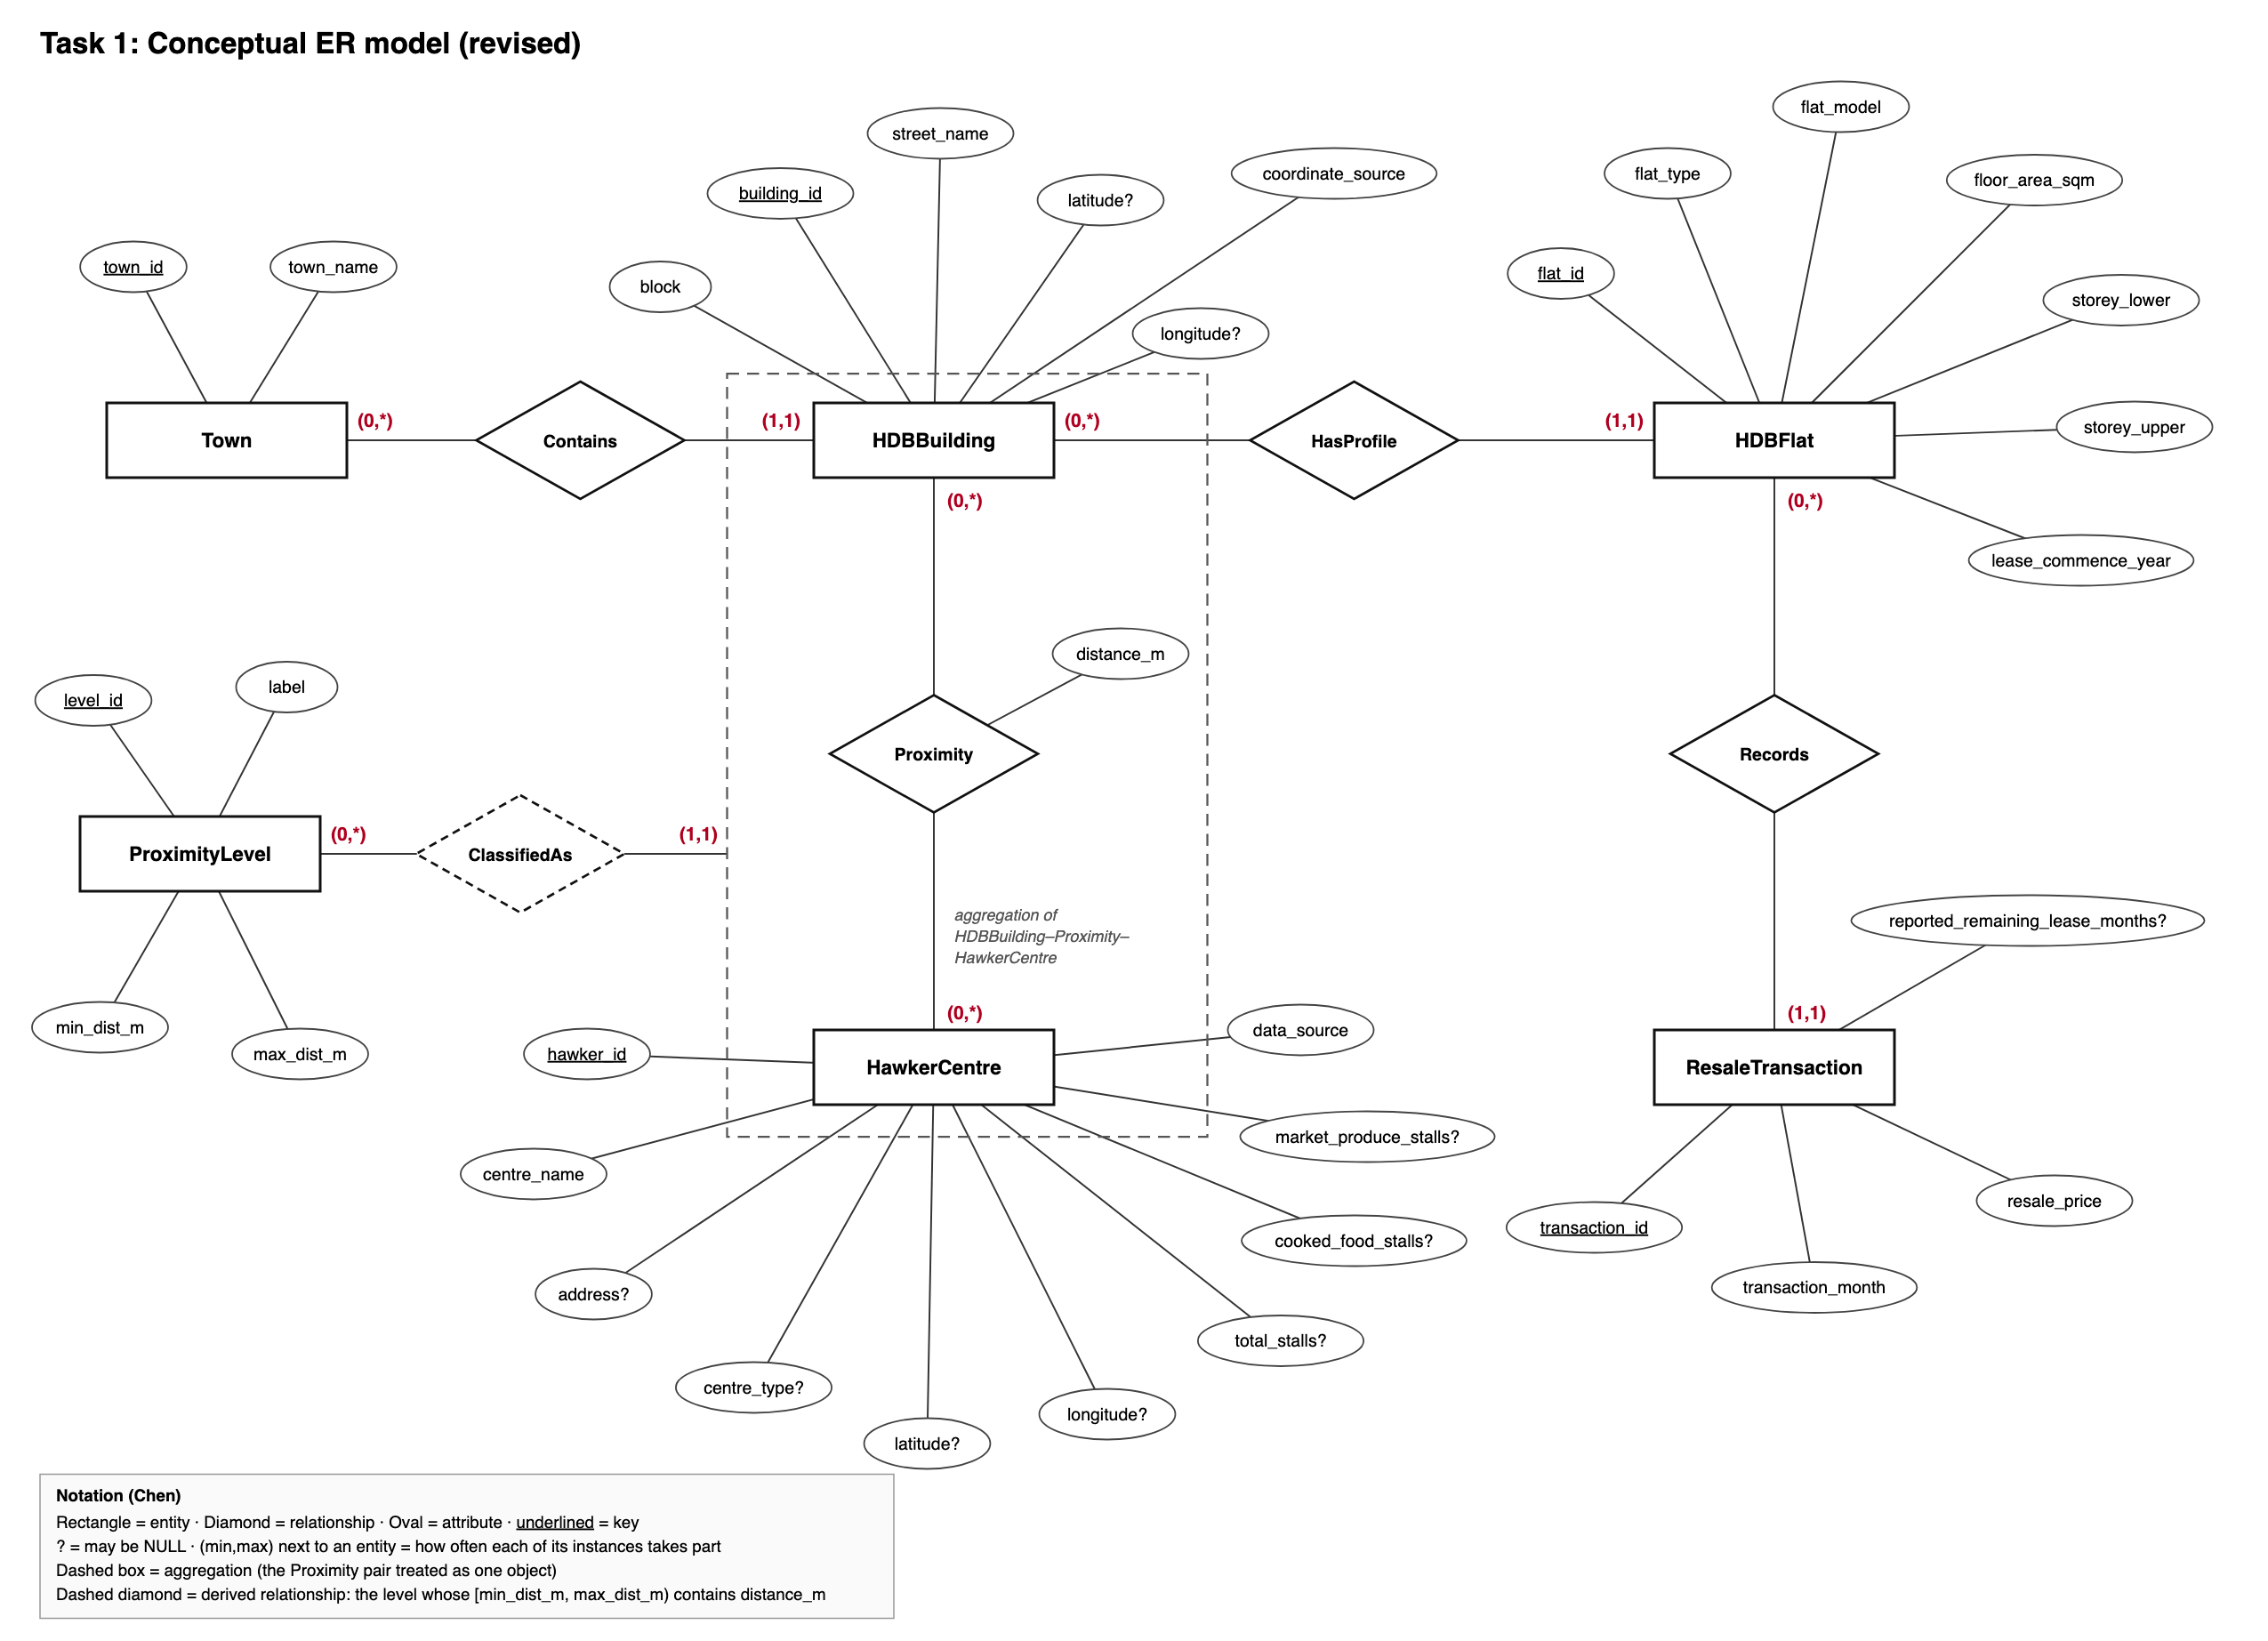
\includegraphics[width=0.95\linewidth,height=0.82\textheight,keepaspectratio]{figures/er_diagram.png}
\caption{Complete ER diagram for the revised design (keys and $(\mathrm{min},\mathrm{max})$ cardinalities).}
\label{fig:er}
\end{figure}
\end{landscape}

\subsection{Logical schema and data dictionary}
One-to-many relationships become foreign keys.
Proximity becomes table \texttt{proximity} keyed by $(\texttt{building\_id},\texttt{hawker\_id})$.
We derive the proximity level from the distance intervals to avoid storing the same classification twice.
Queries obtain the level by joining \texttt{proximity\_level} on $\texttt{min\_dist\_m} \le \texttt{distance\_m} < \texttt{max\_dist\_m}$.
We also store just one distance measure, since estimated walking distance is a fixed multiple of straight-line distance.

Table~\ref{tab:dict} summarises the seven relations.
The full \texttt{CREATE TABLE} script is in Appendix~\ref{app:schema} (\texttt{sql/schema.sql}).

\begin{table}[H]
\centering
\caption{Seven-table data dictionary (revised schema).}
\label{tab:dict}
\footnotesize
\begin{tabularx}{\textwidth}{@{}p{3.2cm}p{3.3cm}X@{}}
\toprule
Table & Primary key & Important attributes / constraints \\
\midrule
\texttt{town} & \texttt{town\_id} & Unique upper-case \texttt{town\_name}. \\
\texttt{hdb\_building} & \texttt{building\_id} & FK to town; unique $(\texttt{block},\texttt{street\_name})$; optional coordinates in Singapore bbox; \texttt{coordinate\_source}. \\
\texttt{hdb\_flat} & \texttt{flat\_id} & FK to building; unique flat profile; seven flat types; positive area; storey range; lease year 1960--2100. \\
\texttt{resale\_transaction} & \texttt{transaction\_id} & FK to flat; month on first of month $\ge$ 1990-01-01; positive price; optional reported remaining lease (months). \\
\texttt{hawker\_centre} & \texttt{hawker\_id} & Unique name; type HC/MHC/MK; stall counts; coordinates; data source tag. \\
\texttt{proximity\_level} & \texttt{level\_id} & Unique label; half-open distance interval; GiST exclusion prevents overlap. \\
\texttt{proximity} & \texttt{building\_id}, \texttt{hawker\_id} & FKs to building and hawker; non-negative \texttt{distance\_m}. \\
\bottomrule
\end{tabularx}
\end{table}

\paragraph{Why \texttt{lease\_commence\_year} stays on the flat.}
Across all five resale files, three buildings have two different lease commence years.
Keeping the year on the flat profile preserves these differences within a building.

\paragraph{Normalisation.}
We separate town names, building addresses, flat profiles and transactions so that each fact is stored at its appropriate level.
Town name, building address and the complete flat profile are declared unique alternate keys.
For proximity, the building--hawker pair determines distance, while the non-overlapping intervals determine its classification.
Under these modelled dependencies, each non-trivial determinant is a candidate key, giving a BCNF design.
The surrogate keys simplify joins, and the corresponding uniqueness constraints preserve the natural identifiers (Appendix~\ref{app:schema}).
No Task~4 performance indexes are created in the schema script---only the indexes PostgreSQL creates for PRIMARY KEY, UNIQUE and EXCLUDE.

\subsection{Implementation}
The schema is created in one transaction by \texttt{Task 1/revised/schema.sql} (copied to Appendix~\ref{app:schema}).
Bulk load uses server-side \texttt{COPY} from the seven CSVs of a chosen step (\texttt{load\_data.sql}).
Constraints reject invalid states at load time (canonical text, flat types, positive prices and areas, Singapore coordinate bounds, non-overlapping levels).

\section{Task 2 --- Data Acquisition and Population}

\subsection{Automated ETL}
The executable ETL is \texttt{Task 2/notebook/Data Systems Task 2 (revised).ipynb}.
It reads the selected resale file(s), the NEA hawker list, \texttt{hawker\_geo.csv} and \texttt{hdb.csv}, validates against Task~1 constraints, and writes one CSV per table under \texttt{data/processed\_steps/step\_$k$/}, ready for \texttt{COPY}.
Missing values are filled from supplementary sources or retained as NULL where the schema permits. Transactions are retained when coordinates are unavailable.
The \texttt{STEP} setting selects how many resale files to process, using the same code for all five datasets.

\subsection{Transformations and computations}
Table~\ref{tab:etl} summarises the transformations. Postal codes provide a better initial match between the hawker files than centre names, matching 104 of 107 centres compared with 17 by name.

\begin{table}[H]
\centering
\caption{Key ETL transformations.}
\label{tab:etl}
\footnotesize
\begin{tabular}{@{}p{2.2cm}p{5.4cm}p{5.6cm}@{}}
\toprule
Input & Transformation & Reason \\
\midrule
Resale & Trim/upper-case town, block, street, type, model & Canonical spelling \\
Resale & \texttt{month} $\to$ DATE; storey range $\to$ two integers & Atomic typed columns \\
Resale & Remaining lease text $\to$ months; NULL if column absent & Consistent unit; missing values retained \\
Resale & \texttt{MULTI GENERATION} $\to$ \texttt{MULTI-GENERATION} & Match the schema spelling \\
Resale & Split into town, building, flat, transaction + surrogate keys & Remove repetition \\
Buildings & Coordinates: \texttt{hdb.csv}, then OneMap, else NULL & Offline first \\
Hawkers & Join gov list and geo file on postal code & Stable join key \\
Proximity & Haversine $\times 1.5$; keep $<2{,}400\,\mathrm{m}$ & Task~1 walking estimate \\
\bottomrule
\end{tabular}
\end{table}

\subsection{Five cumulative database sizes}
Because Q1 needs a three-year window, step~1 starts from the January~2017 onwards file rather than 2015--2016.
Older files are then added in reverse chronological order; each step keeps prior sales (Table~\ref{tab:steps}).
At step~5 the quality report records 987{,}686 transactions spanning 1990-01 to 2026-09, 10{,}014 buildings, 146{,}935 flat profiles, 131 hawker centres and 30{,}908 proximity pairs.

\begin{table}[H]
\centering
\caption{Cumulative ETL steps (sales counts from quality reports / Task~3 summary).}
\label{tab:steps}
\begin{tabular}{@{}clrr@{}}
\toprule
Step & File added & Period covered & Sales \\
\midrule
1 & Jan 2017 onwards & 2017--2026 & 241{,}483 \\
2 & Jan 2015 -- Dec 2016 & 2015--2026 & 278{,}636 \\
3 & Mar 2012 -- Dec 2014 & 2012--2026 & 330{,}839 \\
4 & 2000 -- Feb 2012 & 2000--2026 & 700{,}490 \\
5 & 1990 -- 1999 & 1990--2026 & 987{,}686 \\
\bottomrule
\end{tabular}
\end{table}

\subsection{Coverage gaps that affect proximity queries}
At full load, 140 buildings have NULL coordinates (\texttt{coordinate\_source = none}) and therefore no proximity pairs.
Another 10 matched OneMap on block number only.
One hawker centre lacks coordinates.
Of 10{,}014 buildings, 9{,}246 have at least one hawker within $2{,}400\,\mathrm{m}$; 768 have none.
Sales on buildings without a proximity class remain in the database and contribute to Q1--Q3, but are excluded from Q4--Q6.
Files before 2015 have no \texttt{remaining\_lease} column: 709{,}050 transactions store NULL for reported remaining lease; Q2 derives years from lease commence year instead.

\subsection{Loading issues and fixes}
Client \verb|\copy| failed in our SQL tool (a syntax error at the backslash); we switched to server-side \texttt{COPY} with absolute paths.
Re-running \texttt{schema.sql} without a prior drop aborted on \texttt{schema "housing" already exists}; reloads now start with \texttt{DROP SCHEMA housing CASCADE}.
One incomplete load left \texttt{proximity} empty until reloaded.
Surrogate keys are renumbered every ETL run, so each step reloads all seven tables rather than appending.
Validation identified 279 rows using the older \texttt{MULTI GENERATION} spelling, which we mapped to the schema spelling. Moving raw files under \texttt{data/raw/} also required correcting the notebook's input paths.

\subsection{Supplementary material}
The revised notebook is the executable deliverable for Task~2.
Each step folder also contains \texttt{data\_quality\_report.txt} documenting row counts, key checks, constraint violations (all zero in the saved validation reports) and NULL profiles.

\section{Task 3 --- Queries, Results and Insights}

Unless noted otherwise, result screenshots and insights use \textbf{step~1} (241{,}483 sales, 2017--2026).
Q2--Q5 include older, unadjusted prices as the dataset grows, so we use step~1 for their interpretation. Q1 and Q6 retain the same 2022--2024 window at every step.
Full SQL for Q1--Q6 is in Appendix~\ref{app:queries} (\texttt{sql/queries.sql}).
Screenshots show the first rows returned in the measurement notebook; complete step~1 CSVs are under \texttt{Task 3/results/query\_results\_step1/}.

\subsection{Q1 --- Price per square metre across towns}
\paragraph{Question.}
Average price per m$^2$ for 4-room and 5-room flats sold in calendar years 2022--2024, by town and flat type.
\paragraph{SQL.} Appendix~\ref{app:queries}, query Q1.
\paragraph{Result.} Figure~\ref{fig:q1}.

\begin{figure}[H]
\centering
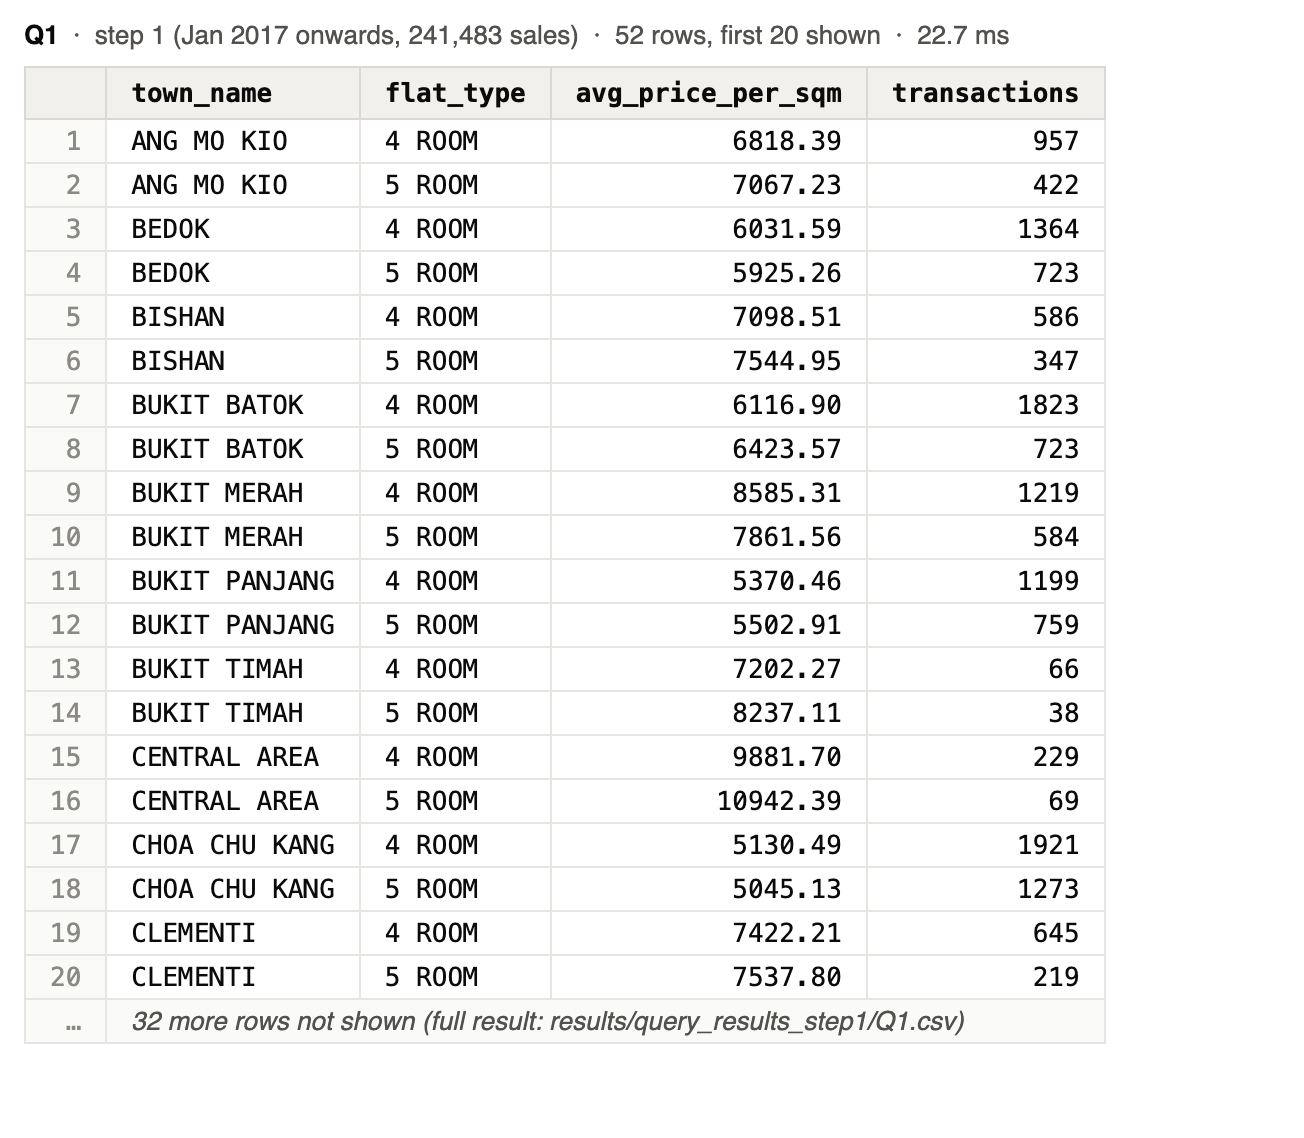
\includegraphics[width=0.92\textwidth]{figures/q1_result.png}
\caption{Q1 result excerpt (step~1).}
\label{fig:q1}
\end{figure}

\paragraph{Insight.}
For four-room flats, price per m$^2$ in 2022--2024 is nearly twice as high in Central Area ($\approx$9{,}882) and Queenstown ($\approx$9{,}353) as in Choa Chu Kang ($\approx$5{,}130).
Five-room flats cost more per m$^2$ than four-room flats in only 10 of 26 towns in this extract.


\subsection{Q2 --- Remaining lease versus transaction price}
\paragraph{Question.}
We estimate remaining lease in years as
\[
99 - (\text{sale year} - \text{lease commence year}).
\]
The query groups sales into lease buckets and reports median resale price, average price per m$^2$ and transaction volume for each town and bucket.
\paragraph{SQL.} Appendix~\ref{app:queries}, query Q2.
\paragraph{Result.} Figure~\ref{fig:q2}.

\begin{figure}[H]
\centering
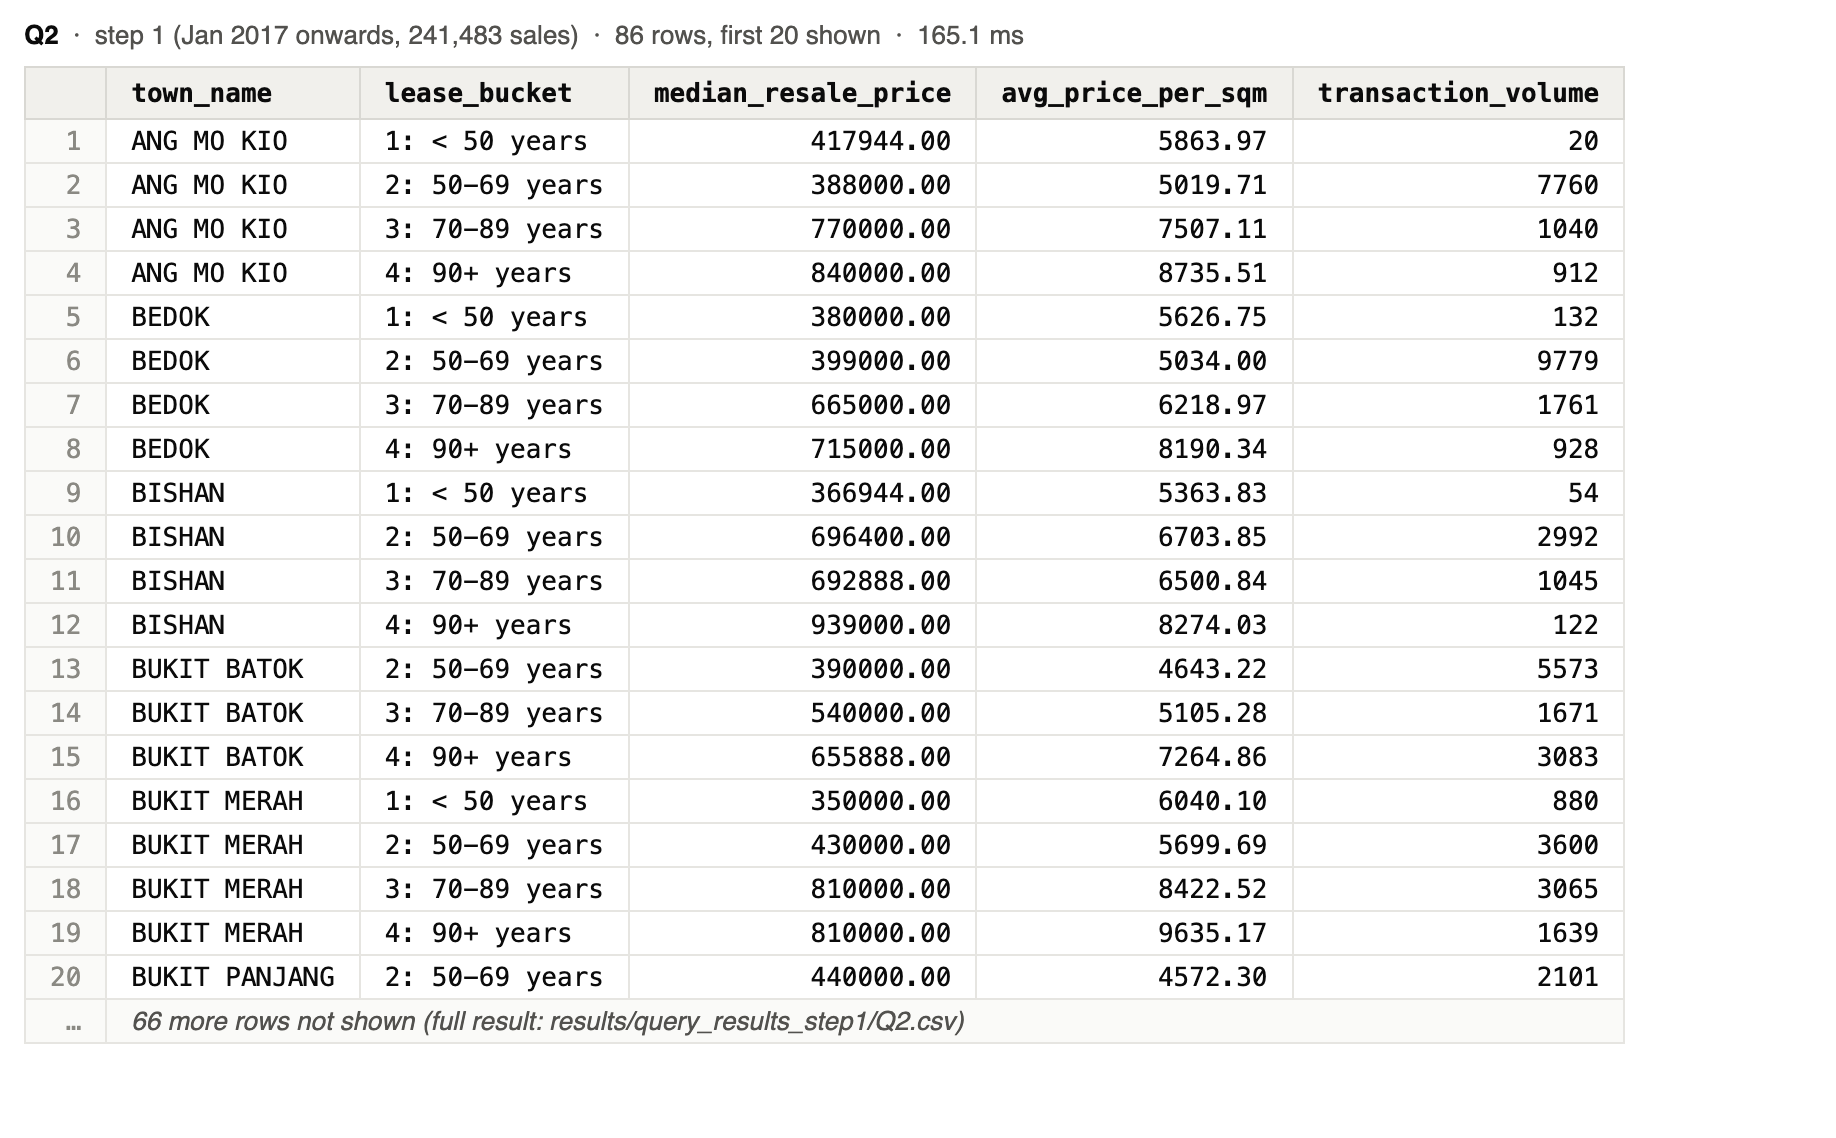
\includegraphics[width=0.92\textwidth]{figures/q2_result.png}
\caption{Q2 result excerpt (step~1).}
\label{fig:q2}
\end{figure}

\paragraph{Insight.}
In 19 of 20 towns with both buckets present, flats with $90+$ years of lease left have a higher median price than those with 50--69 years.
The under-50 bucket is too small in many towns to interpret.
Across the full dataset, a few older approval-date sales yield estimated remaining leases of 100--101 years. This reflects a limitation of deriving lease duration from the recorded sale year.

\subsection{Q3 --- Resale price for towns with large flats}
\paragraph{Question.}
Identify the ten towns with the highest \emph{transaction-weighted} average floor area of 3-room flats sold (\texttt{AVG(floor\_area\_sqm)} over sales, not over distinct flat profiles).
For those towns, return the maximum 3-room resale price in each sale year.
\paragraph{SQL.} Appendix~\ref{app:queries}, query Q3.
\paragraph{Result.} Figure~\ref{fig:q3}.

\begin{figure}[H]
\centering
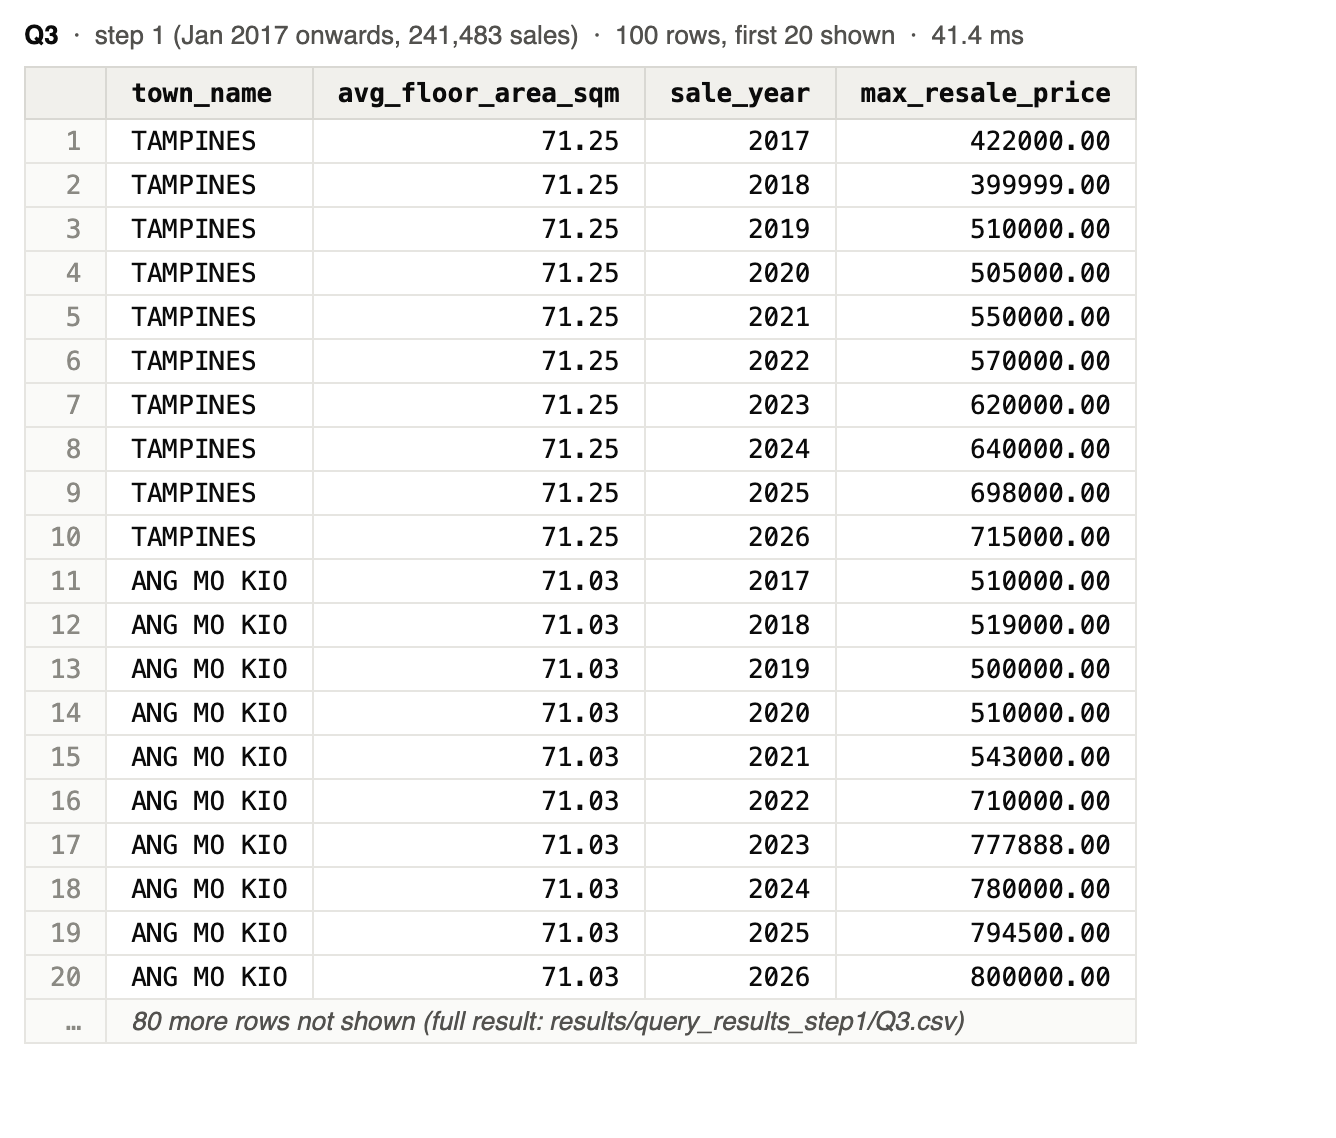
\includegraphics[width=0.92\textwidth]{figures/q3_result.png}
\caption{Q3 result excerpt (step~1).}
\label{fig:q3}
\end{figure}

\paragraph{Insight.}
The ten towns differ by less than $3\,\mathrm{m}^2$ on average floor area.
Their highest yearly prices increased by about 18\% to 81\% between 2017 and the available January--September 2026 sales.
Because the average is sale-weighted, towns with many small 3-room sales can rank differently from a profile-based average.

\subsection{Q4 --- Hawker centre proximity effect}
\paragraph{Question.}
Compare average resale price when the building's \emph{nearest} hawker (any type) is in level~1 versus level~3, by town and flat type; keep only groups with sales in both classes.
\paragraph{SQL.} Appendix~\ref{app:queries}, query Q4.
\paragraph{Result.} Figure~\ref{fig:q4}.

\begin{figure}[H]
\centering
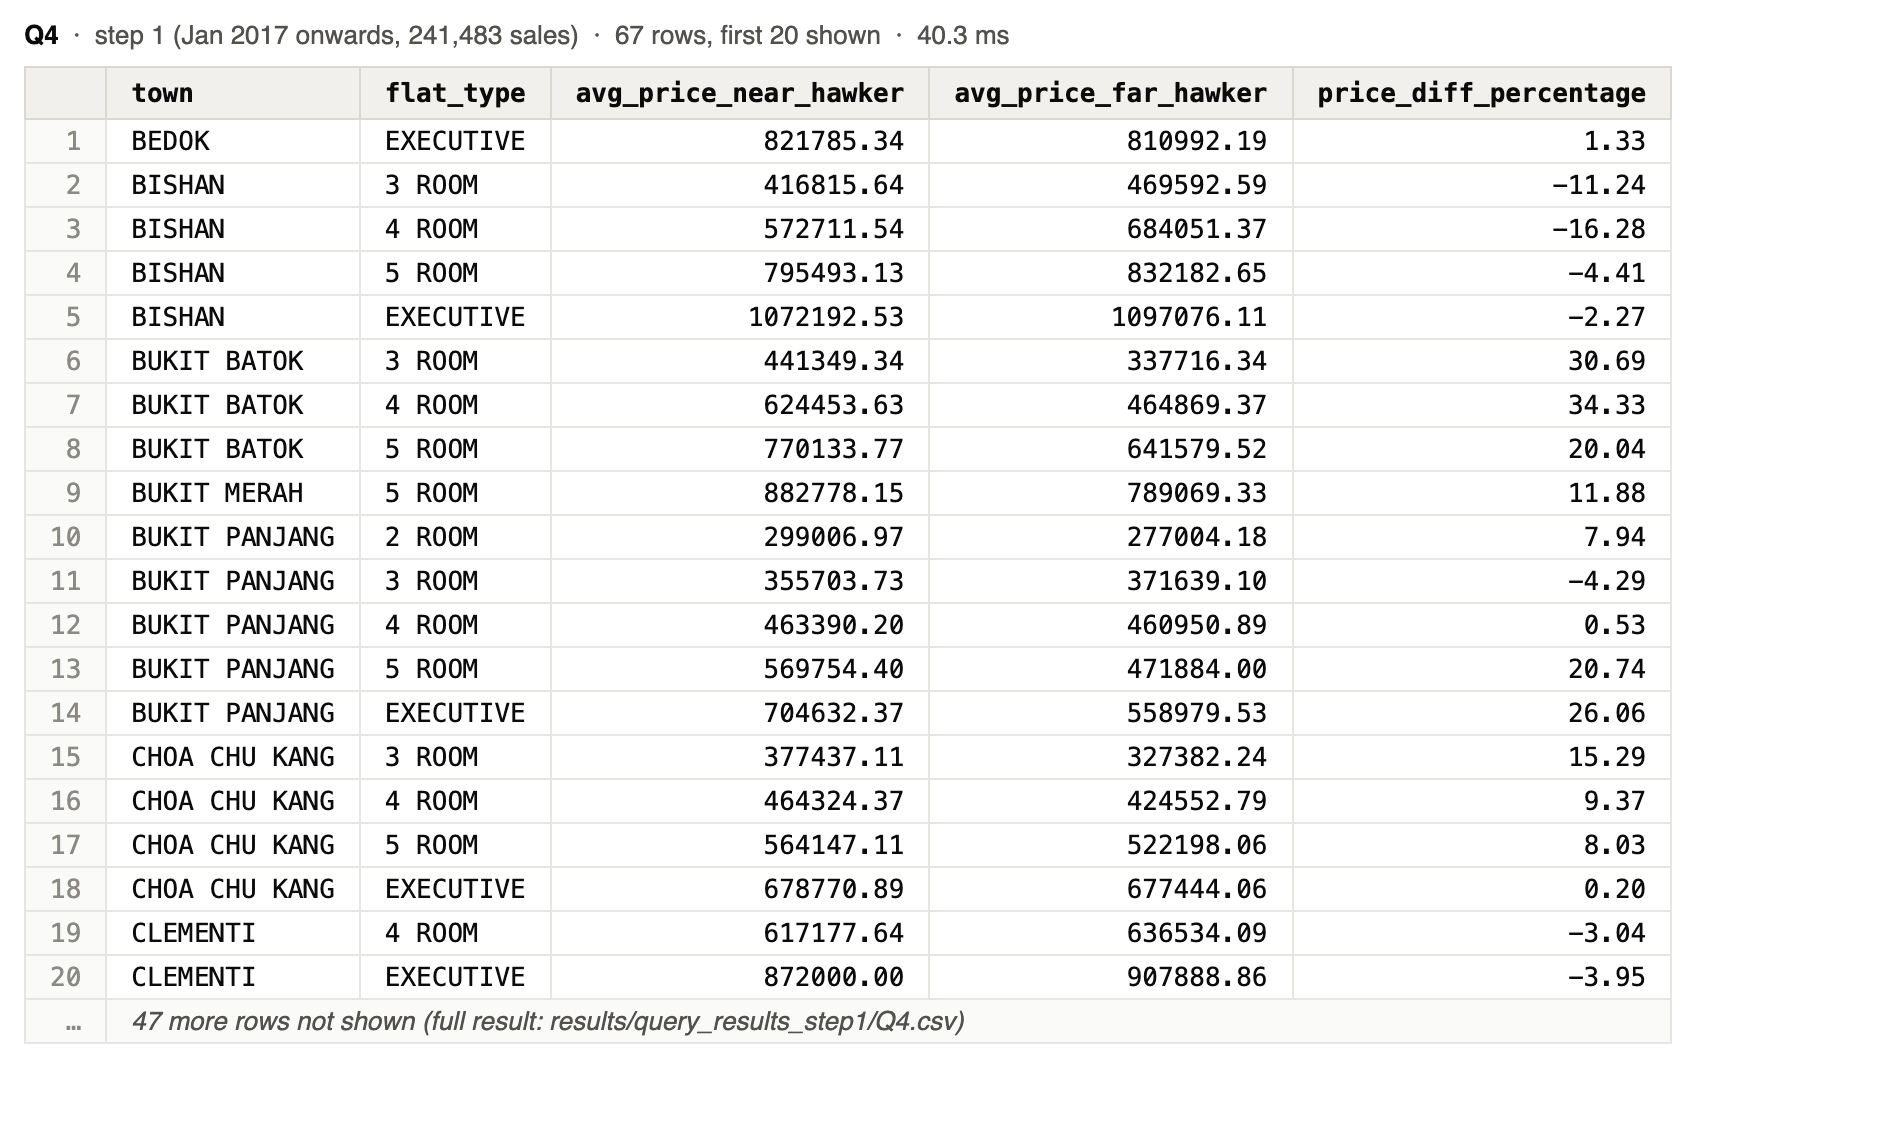
\includegraphics[width=0.92\textwidth]{figures/q4_result.png}
\caption{Q4 result excerpt (step~1).}
\label{fig:q4}
\end{figure}

\paragraph{Insight.}
Near flats cost more than far ones in 42 of 67 town$\times$type groups and less in 25 (median gap about $+3\%$).
The mixed price differences do not establish a causal effect of proximity. The query does not control for other flat attributes or differences between estates.
Buildings without any centre within $2{,}400\,\mathrm{m}$ are absent from the comparison.

\subsection{Q5 --- Town-level price near fresh-market hawkers}
\paragraph{Question.}
For flats whose nearest hawker with \texttt{market\_produce\_stalls > 0} falls in a proximity class, report average resale price by town and class.
Keep towns whose overall average for these flats exceeds SGD~450{,}000 (chosen so the result is neither empty nor all towns at every database size).
\paragraph{SQL.} Appendix~\ref{app:queries}, query Q5.
\paragraph{Result.} Figure~\ref{fig:q5}.

\begin{figure}[H]
\centering
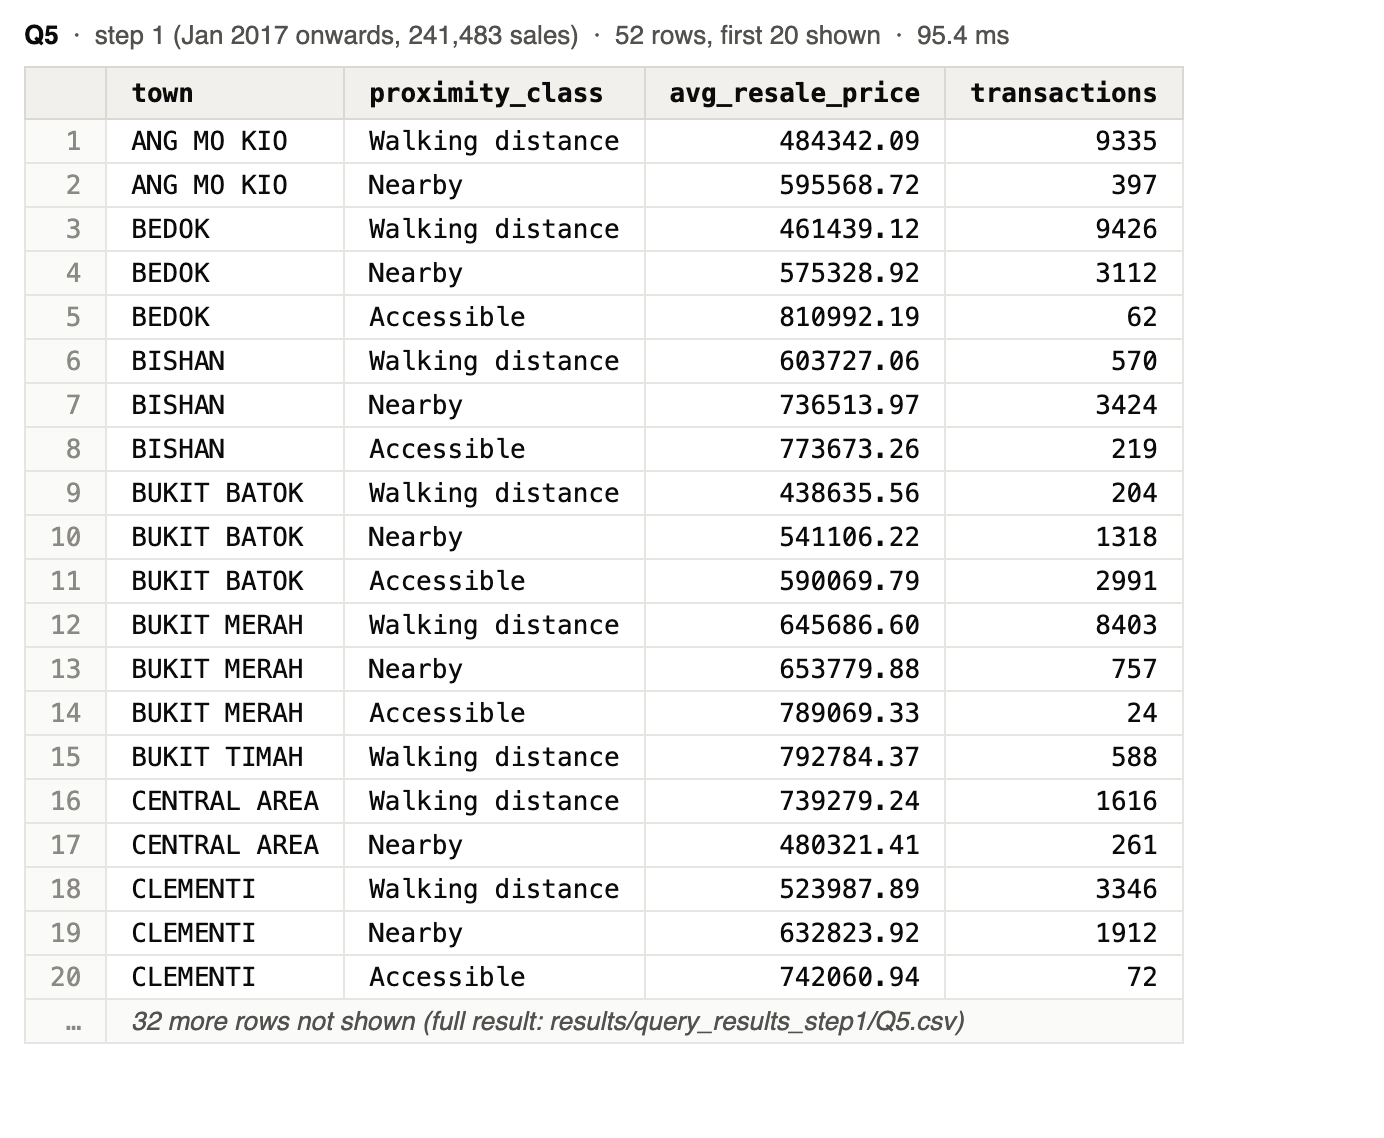
\includegraphics[width=0.92\textwidth]{figures/q5_result.png}
\caption{Q5 result excerpt (step~1).}
\label{fig:q5}
\end{figure}

\paragraph{Insight.}
With a SGD~450{,}000 budget, 20 of 22 towns near a fresh-market centre pass at step~1.
In 12 of 17 towns with both a walking-distance class and another class, the walking-distance class has the lowest average price. Estate age may contribute to this pattern, but the query does not test that explanation.
An initial budget of SGD~600{,}000 returned no towns at steps~4--5, where older sales lowered the averages. We therefore used SGD~450{,}000 for all reported measurements.
Unlike Q4, ``nearest'' here means nearest market-produce hawker, not nearest hawker of any type.

\subsection{Q6 --- Own query (joins all seven tables)}
\paragraph{Question.}
For 4-room flats sold in 2022--2024, does the \emph{type} of the nearest hawker centre (HC / MHC / MK / UNKNOWN) relate to average price per m$^2$, by proximity class of that nearest centre?
\paragraph{SQL.} Appendix~\ref{app:queries}, query Q6. The query joins \texttt{resale\_transaction}, \texttt{hdb\_flat}, \texttt{hdb\_building}, \texttt{town}, \texttt{proximity}, \texttt{hawker\_centre} and \texttt{proximity\_level}.
\paragraph{Result.} Figure~\ref{fig:q6}.

\begin{figure}[H]
\centering
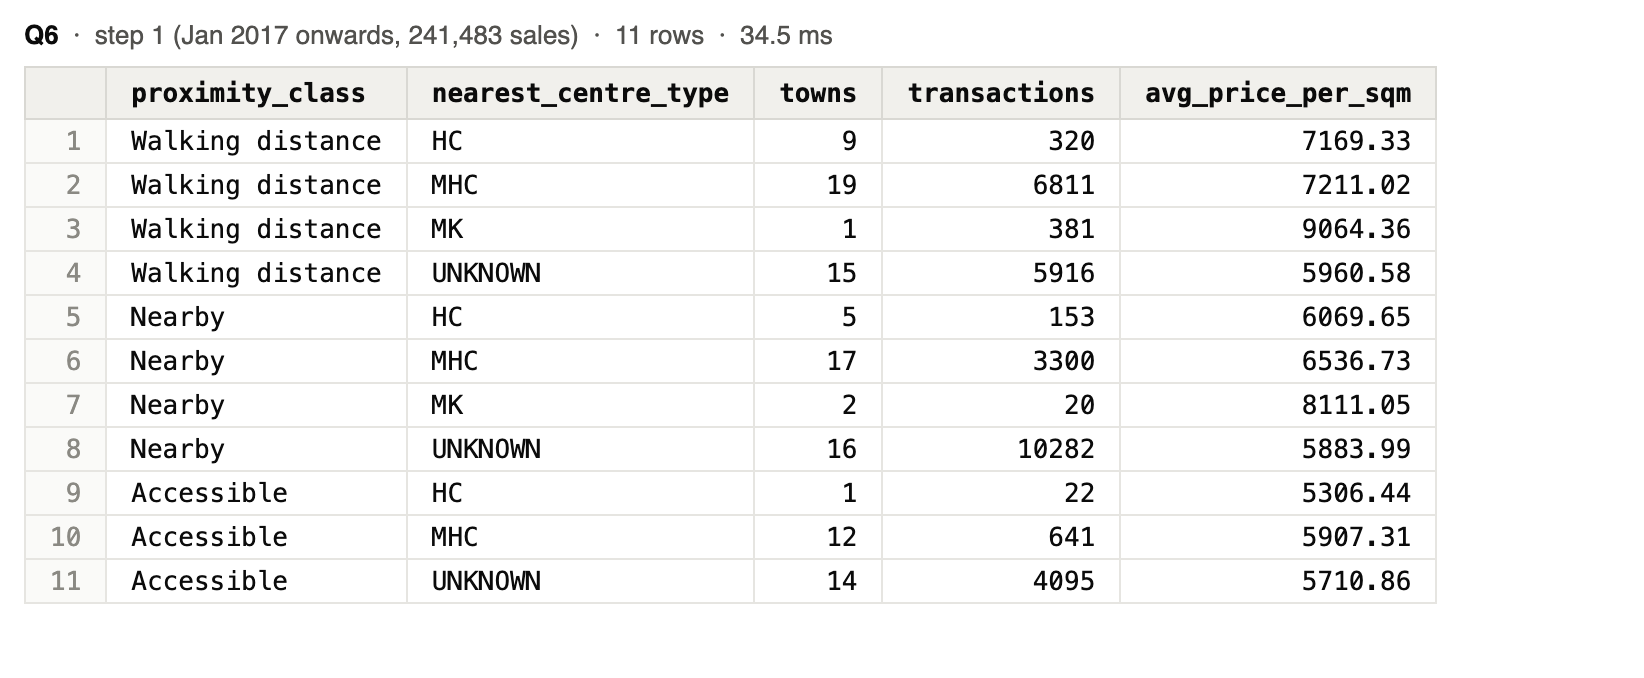
\includegraphics[width=0.85\textwidth]{figures/q6_result.png}
\caption{Q6 result (step~1).}
\label{fig:q6}
\end{figure}

\paragraph{Insight.}
For 4-room sales in 2022--2024, average price per m$^2$ near a market-and-hawker centre (MHC) falls from about 7{,}211 in walking distance to about 5{,}907 in the accessible class in this extract.
These averages describe the selected sales under the nearest-centre definition. Differences in flat and estate characteristics remain uncontrolled.

\section{Task 3 --- Performance Across Database Sizes}

\subsection{Measurement protocol}
We run each of Q1--Q6 five times at each of the five cumulative sizes, giving 150 timing records in \path{Task 3/results/task3_measurements.csv}. The measurement loop has no separate warm-up, although the notebook executes the queries in its earlier results section.
Runtime is the client-observed time around SQL execution and fetching all result rows.
Database size and housing size are recorded with each block in the measurement file; Table~\ref{tab:t3perf} uses the per-step averages from \texttt{task3\_summary.csv}.
The later Task~4 environment snapshot records PostgreSQL~18.4 on macOS arm64 with 10 CPUs. Task~3 has no equivalent saved environment snapshot, so we cannot verify every setting against that later record.

\subsection{Average runtime by size}
Table~\ref{tab:t3perf} reports mean runtime in milliseconds (five runs).
Figure~\ref{fig:t3chart} plots runtime against database size for each query.

\begin{table}[H]
\centering
\caption{Mean runtime (ms) of Q1--Q6 over five timed runs at each database size. Sales and DB size from \texttt{task3\_summary.csv}.}
\label{tab:t3perf}
\footnotesize
\begin{tabular}{@{}rrrrrrrrr@{}}
\toprule
Step & Sales & DB (MB) & Q1 & Q2 & Q3 & Q4 & Q5 & Q6 \\
\midrule
1 & 241{,}483 & 44.18 & 22.40 & 163.38 & 40.53 & 39.77 & 93.44 & 34.61 \\
2 & 278{,}636 & 47.54 & 23.29 & 193.04 & 47.80 & 44.16 & 106.37 & 34.97 \\
3 & 330{,}839 & 53.73 & 20.96 & 231.12 & 68.88 & 47.55 & 126.10 & 30.98 \\
4 & 700{,}490 & 83.03 & 20.81 & 314.67 & 141.08 & 58.42 & 155.28 & 31.38 \\
5 & 987{,}686 & 104.87 & 22.28 & 412.19 & 217.83 & 70.58 & 226.61 & 33.47 \\
\bottomrule
\end{tabular}
\end{table}

\begin{figure}[H]
\centering
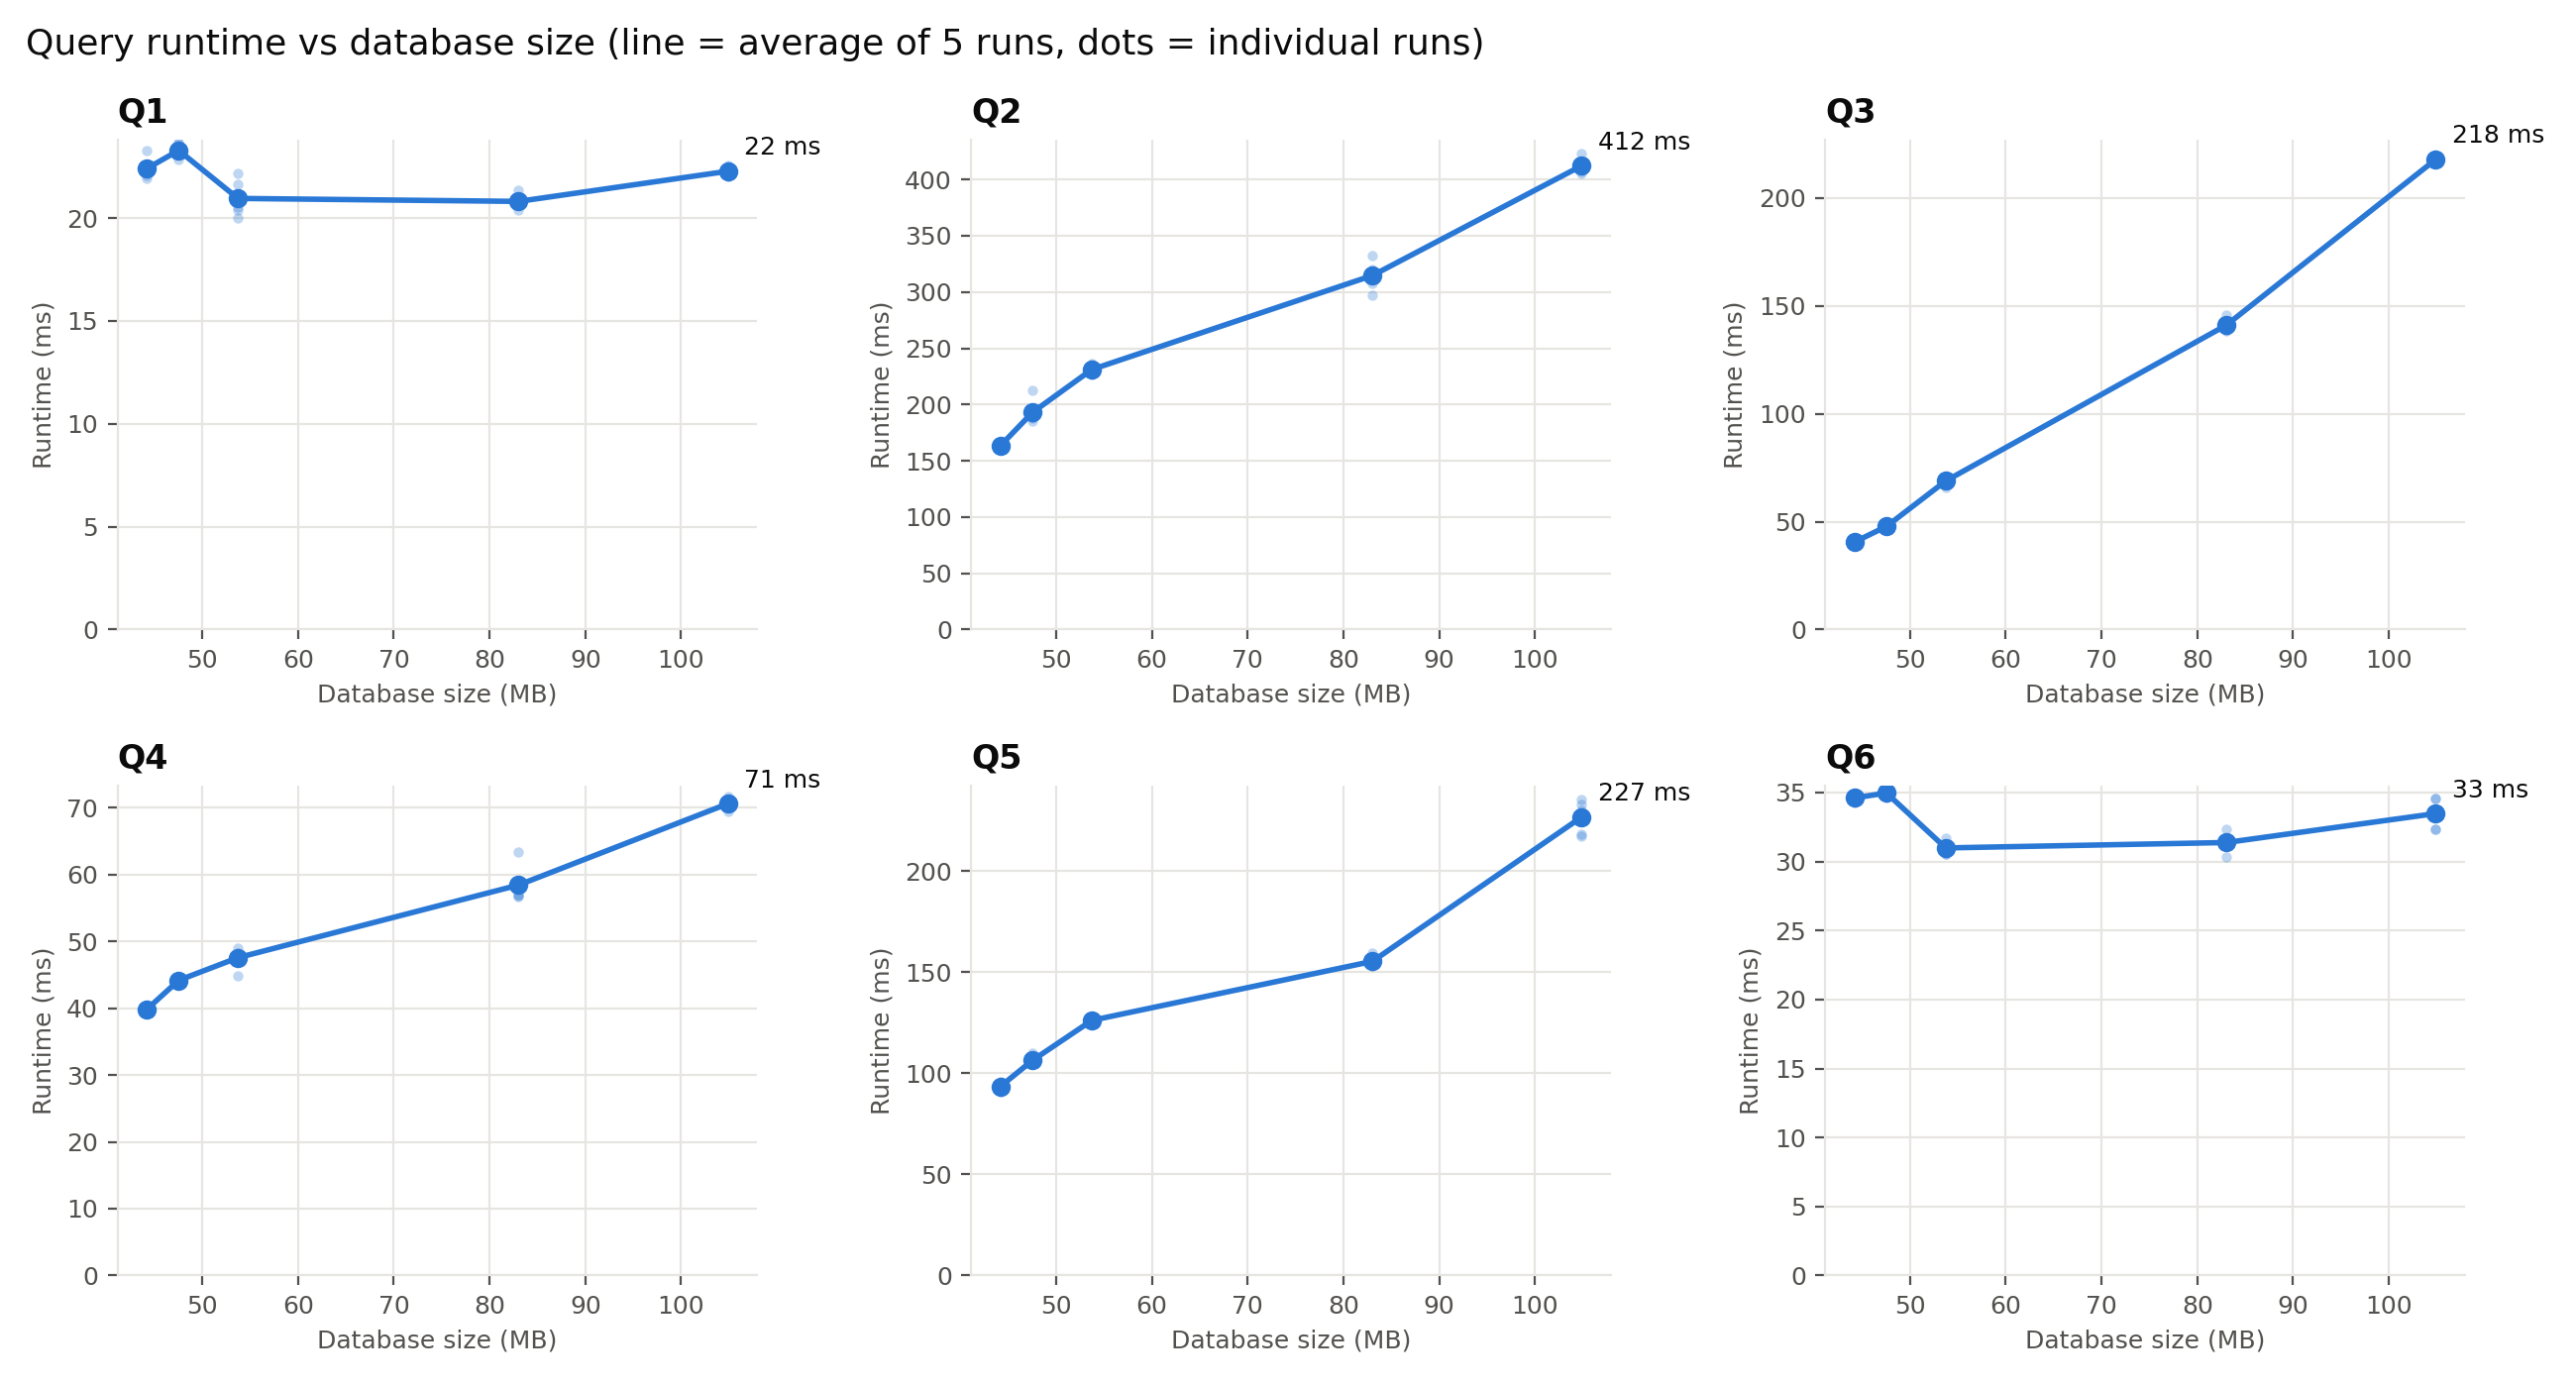
\includegraphics[width=\textwidth]{figures/task3_runtime_vs_size.png}
\caption{Query runtime versus database size (Task~3). Lines connect the five-run means, and dots show individual runs.}
\label{fig:t3chart}
\end{figure}

\subsection{Discussion}
\paragraph{Observed scaling.}
From step~1 to step~5, sales grow by about $4.1\times$ while database size roughly doubles.
Q2 and Q3 grow strongly with size (Q2 about $2.5\times$, Q3 about $5.4\times$).
Q4 and Q5 grow more slowly than the sales count.
Q1 remains around 21--23~ms and Q6 around 31--35~ms.

\paragraph{Execution plans.}
Saved Task~4 \texttt{EXPLAIN} plans on the largest database (without the Task~4 index) show that Q1 and Q6 apply a date filter on \texttt{resale\_transaction} and use parallel sequential scans, keeping only about 8.1\% of sales for 2022--2024.
Q2--Q5 read essentially all sales; Q3's \texttt{WITH three\_room} is referenced twice and is materialised, and Q2's large sort spills to disk under default \texttt{work\_mem} (see Task~4 supporting experiments).
The added files contain older sales outside the Q1/Q6 date window, so their selected transaction sets remain fixed. Parallel scans may also help keep their runtimes low. The saved plans explain the work performed on the largest database, while cache effects and background load across the five measurements remain unmeasured.

\paragraph{Implication for indexing.}
Task~3 suggested Q2 and Q3 as first index candidates because they dominate absolute runtime.
Task~4 tests whether indexes can reduce this work. The clearest improvement comes from indexing the date filter in Q1.

\section{Task 4 --- Index Selection and Evaluation}

All final index timings use the largest database (987{,}686 sales) and the unchanged Task~3 queries.
For each query and condition, we perform one untimed warm-up followed by five timed runs, measuring client time around \texttt{execute} and \texttt{fetchall}. We report the mean and sample standard deviation. Percentage changes use the means rounded to two decimal places, following \texttt{task4\_summary.csv}.
The project's ``noticeable'' rule requires both a plan change and an absolute mean change larger than 10\% of the un-indexed mean \emph{and} larger than two un-indexed sample standard deviations.
We use this as a descriptive threshold for interpreting the measurements.

\subsection{What the plans suggest}
Without extra indexes, only Q1 and Q6 filter \texttt{resale\_transaction} on \texttt{transaction\_month}, keeping 80{,}306 of 987{,}686 rows (8.1\%) and discarding the rest (saved plans under \path{Task 4/results/plans/}).
Q2--Q5 read essentially every sale, so an index has little to skip.
An earlier four-index experiment was reported to slow Q1 and led us to test candidates separately. Its original spreadsheet is unavailable, so we retain it only as context for the experimental design.

\subsection{Candidate screening (summary)}
Nine candidates were created one at a time, analysed, timed on Q1--Q6, and dropped
(\path{task4_candidate_screening.csv}, 330 rows).
Percentages compare each candidate to a \emph{pooled} un-indexed baseline of ten runs (before the first and after the last candidate).
Those two baseline blocks disagree---especially Q1 (26.30 vs 21.06~ms) and Q6 (32.89 vs 40.32~ms), the latter including slow end runs of 50.3 and 47.8~ms---so pooled percentages must be read with that drift in mind.
The slow ending baseline inflates the pooled mean, so negative Q6 percentages require caution.

Table~\ref{tab:screen} summarises the screening results.
Only month-based indexes clearly helped Q1 under the noticeability rule.
\texttt{flat\_id} indexes made Q6 much slower when the planner used them.
The remaining indexes on flat type, town and proximity columns had no noticeable effect under the rule.
Figure~\ref{fig:heat} shows the heat map drawn from the same pooled percentages.

\begin{table}[H]
\centering
\caption{Candidate screening on step~5 (pooled baseline). Build time is CREATE only. Source: \texttt{task4\_candidate\_summary.csv}.}
\label{tab:screen}
\footnotesize
\begin{tabular}{@{}clrrll@{}}
\toprule
ID & Index (abbrev.) & Size (MB) & Build (ms) & Q1 vs pool & Verdict \\
\midrule
C1 & B-tree(\texttt{transaction\_month}) & 6.73 & 130.1 & $-35.8\%$ & \textbf{kept} \\
C2 & covering month & 29.73 & 409.4 & $-39.3\%$ & reject (size) \\
C3 & BRIN(\texttt{transaction\_month}) & 0.02 & 23.8 & $-31.8\%$ & not submitted \\
C4 & B-tree(\texttt{flat\_id}) & 9.72 & 202.0 & noise & reject (Q6 $+66.6\%$) \\
C5 & covering \texttt{flat\_id} & 29.73 & 495.0 & noise & reject \\
C6--C9 & type / town / hawker / prox.\ covering & $\le 0.99$ & $\le 29.8$ & noise & reject \\
\bottomrule
\end{tabular}
\end{table}

\begin{figure}[H]
\centering
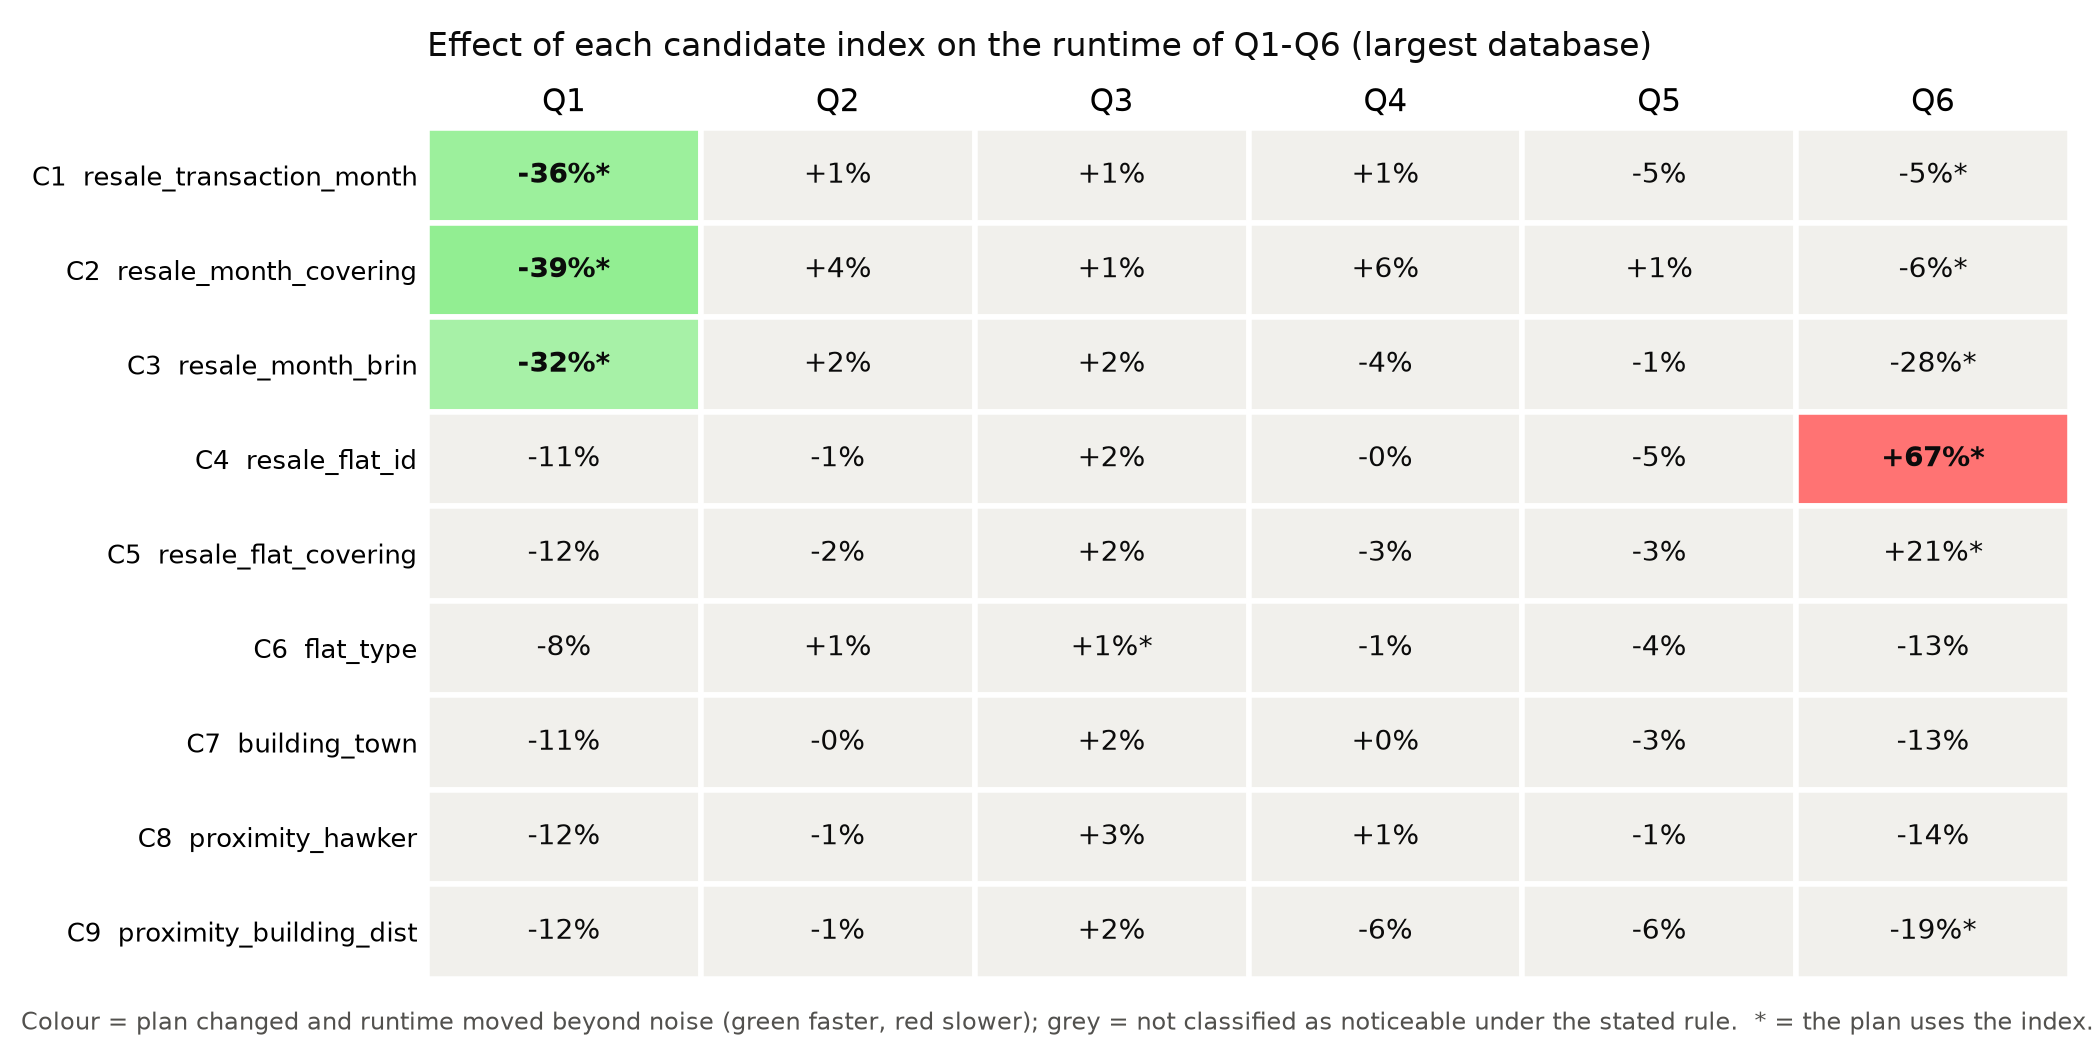
\includegraphics[width=0.95\textwidth]{figures/task4_candidate_screening.png}
\caption{Screening heat map: percent change versus pooled baseline. Asterisk marks index use in the plan. Grey cells fail the project's noticeability rule.}
\label{fig:heat}
\end{figure}

Combinations of C1 with other candidates did not improve Q1 beyond the mid-teens of milliseconds in a way that justified extra indexes (\texttt{task4\_combination\_tests.csv}).
The submitted index is judged from the same-session with/without experiment below, not from screening percentages alone.

\subsection{Final index}
We submit a plain B-tree on the date column (full file in Appendix~\ref{app:indexes}):
\begin{verbatim}
CREATE INDEX idx_resale_transaction_month
    ON housing.resale_transaction (transaction_month);
ANALYZE housing.resale_transaction;
\end{verbatim}
The B-tree targets the selective date filter. Its usefulness is less dependent on physical row ordering than the BRIN alternative.
In screening, the covering B-tree reduced Q1 runtime by a further $0.85\,\mathrm{ms}$ but occupied $4.4\times$ as much space.
BRIN recorded a lower Q6 mean against the drifted baseline, but we chose the B-tree to avoid relying on the ordering produced by the CSV load.

\subsection{Final with/without measurement}
Table~\ref{tab:final} and Figure~\ref{fig:t4bars} show the final comparison from Part~C of the notebook.
Each query was measured five times before and after applying \texttt{indexes.sql}, giving 60 records.
Both conditions contain 987{,}686 transactions. Total database size is 124.01~MB without the index and 130.75~MB with it, compared with 104.87~MB in Task~3 at step~5.
These values use the same database-size function but were recorded at different stages. The files do not establish the cause of the Task~3/4 size difference, so the Task~3 line is a historical reference. We assess the index using the matched Task~4 conditions.

\begin{table}[H]
\centering
\caption{Final index effect on step~5 (mean $\pm$ sample SD, ms). Source: \texttt{task4\_summary.csv}.}
\label{tab:final}
\footnotesize
\begin{tabular}{@{}lrrrl@{}}
\toprule
Query & Without index & With index & Change & Index used \\
\midrule
Q1 & $21.56 \pm 0.25$ & $14.93 \pm 0.32$ & $-30.8\%$ ($1.44\times$) & yes \\
Q2 & $392.17 \pm 3.93$ & $386.40 \pm 5.59$ & $-1.5\%$ (plan unchanged) & no \\
Q3 & $212.18 \pm 0.48$ & $208.10 \pm 0.89$ & $-1.9\%$ (plan unchanged) & no \\
Q4 & $69.97 \pm 0.80$ & $70.32 \pm 0.49$ & $+0.5\%$ (plan unchanged) & no \\
Q5 & $209.47 \pm 6.36$ & $205.62 \pm 2.69$ & $-1.8\%$ (plan unchanged) & no \\
Q6 & $32.62 \pm 1.64$ & $34.61 \pm 0.15$ & $+6.1\%$ & yes \\
\bottomrule
\end{tabular}
\end{table}

\begin{figure}[H]
\centering
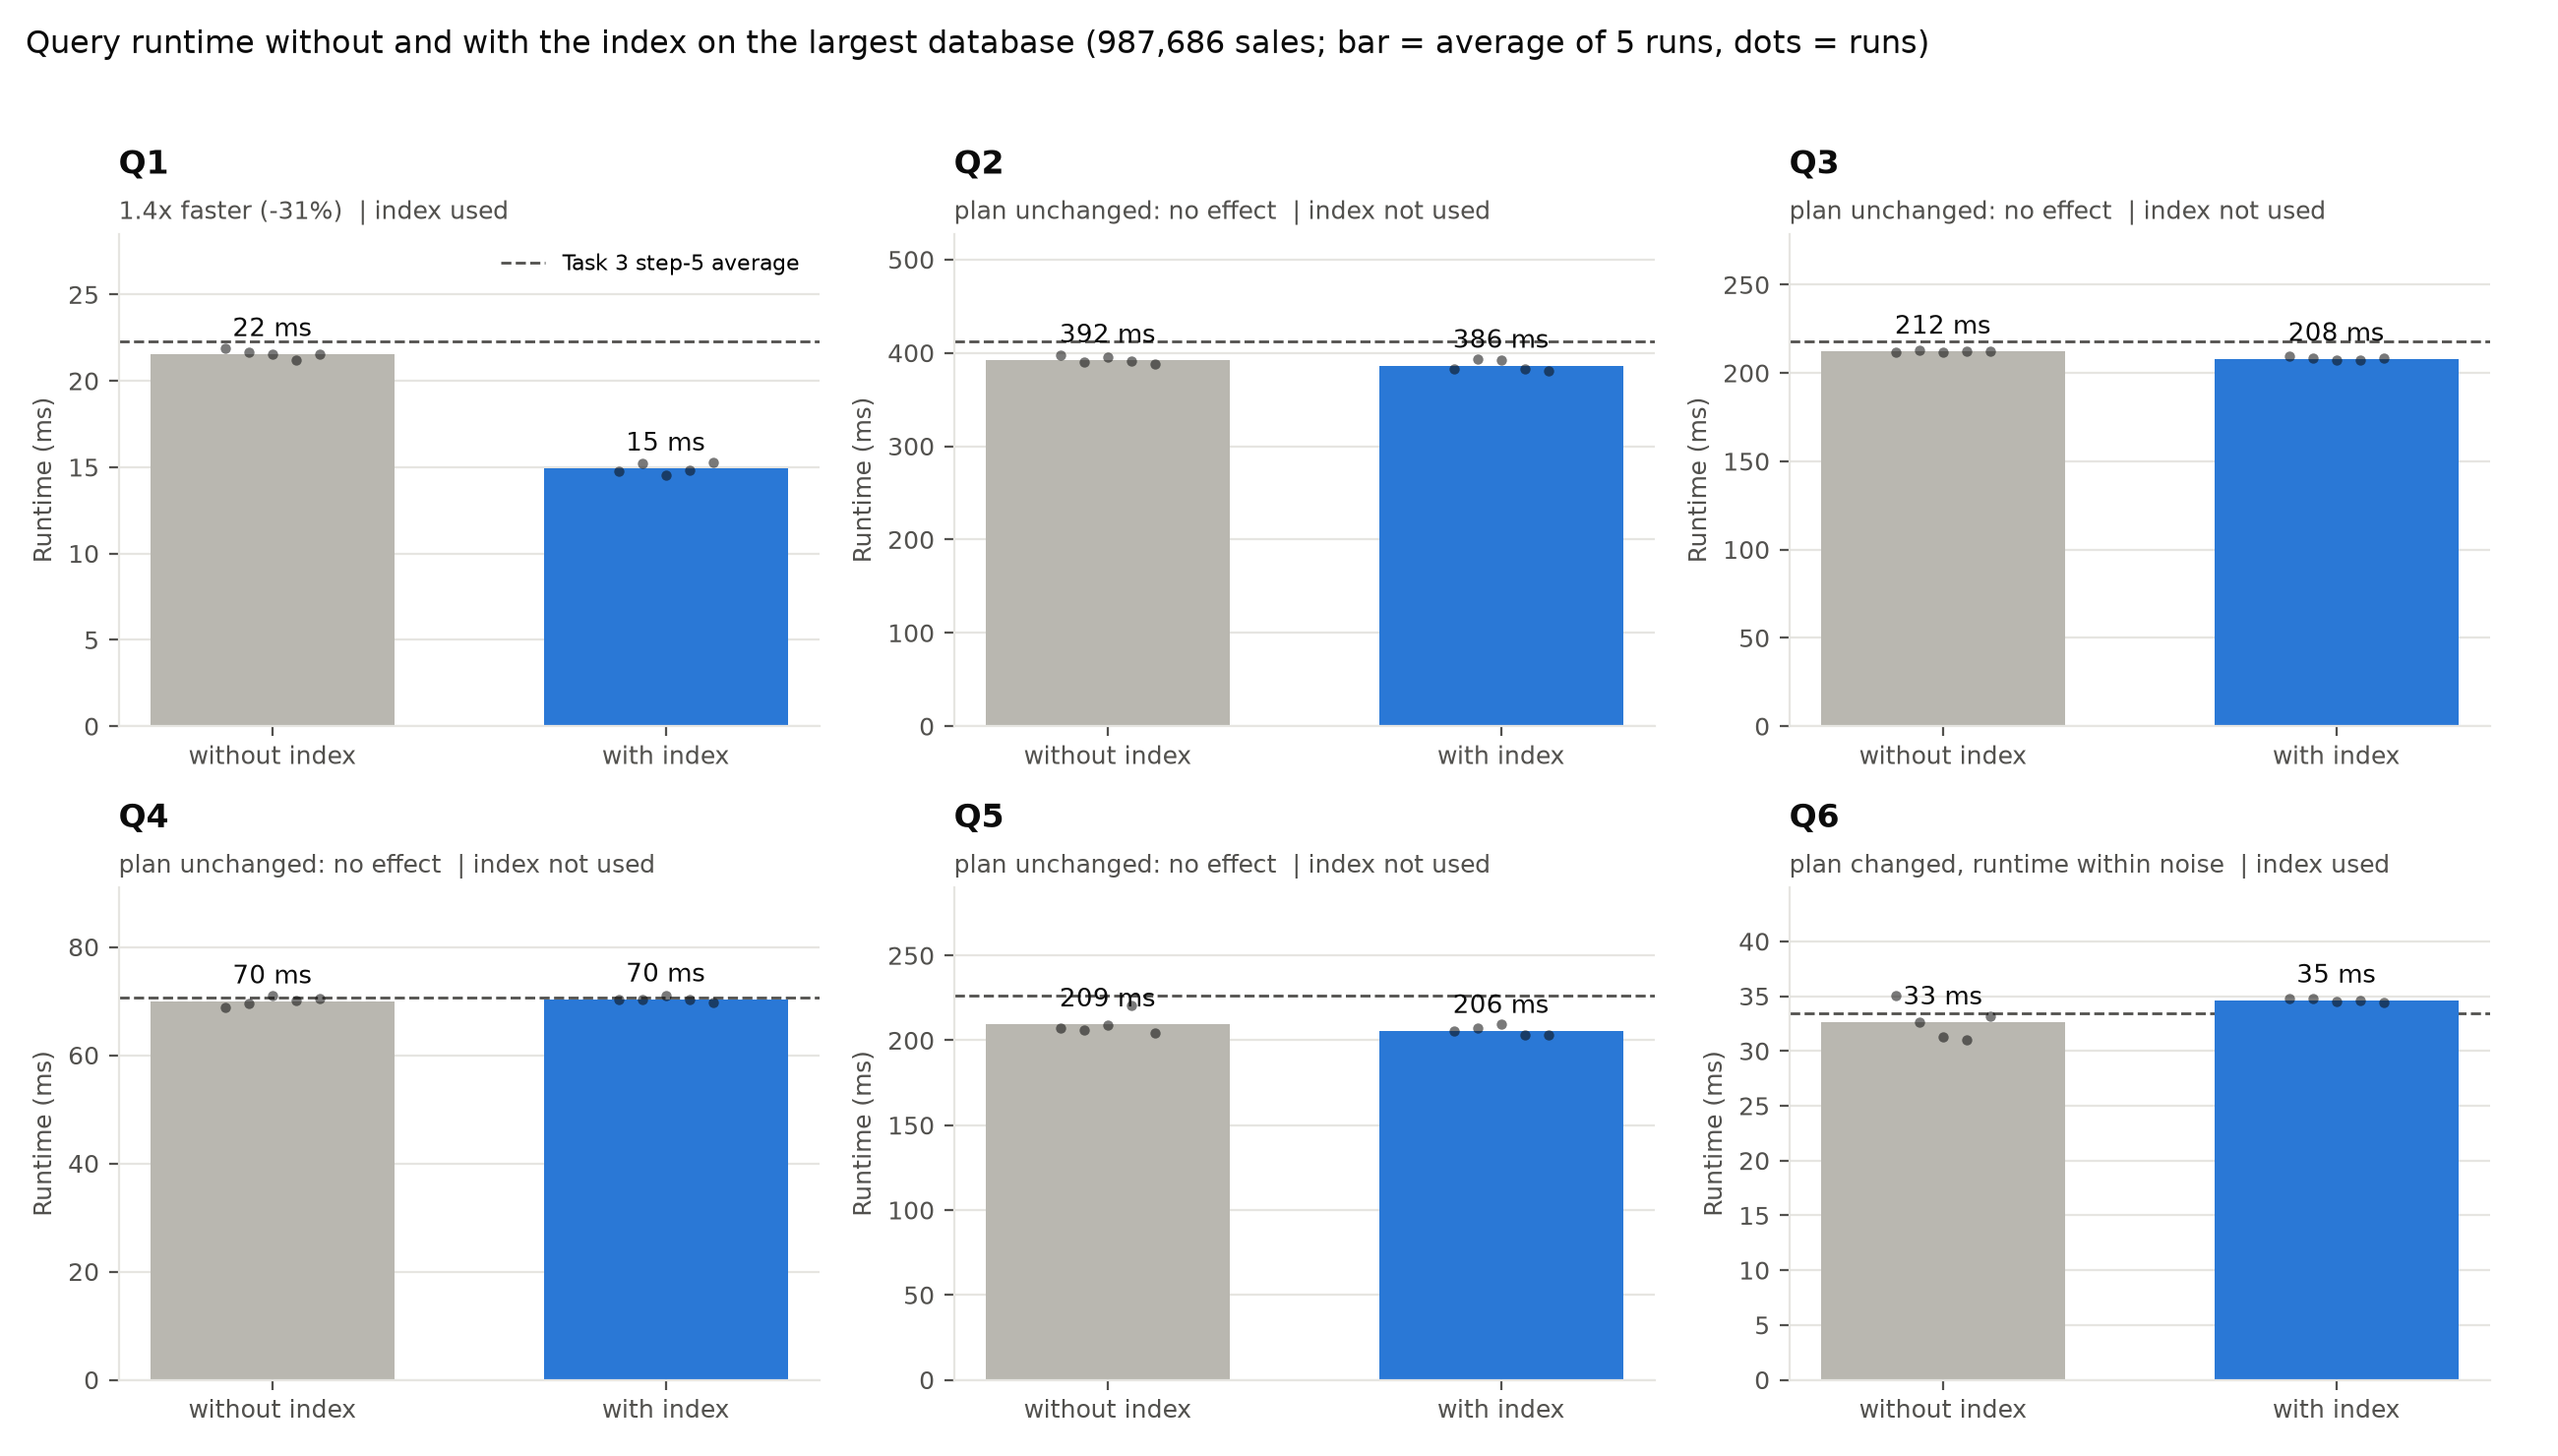
\includegraphics[width=\textwidth]{figures/task4_runtime_with_vs_without_index.png}
\caption{Average client runtime without and with the submitted index (five runs; dots are individual timed runs). Dashed line: Task~3 step~5 average.}
\label{fig:t4bars}
\end{figure}

\paragraph{Q1.}
The plan changes from a parallel sequential scan with a date filter to a parallel bitmap heap scan fed by a bitmap index scan on \texttt{idx\_resale\_transaction\_month}, returning the 80{,}306 matching rows.
Client mean runtime falls by $6.63\,\mathrm{ms}$ ($-30.8\%$).
The saved \texttt{EXPLAIN ANALYZE} plans support this change in access method. Their instrumented server execution times are separate from the client averages reported here.

\paragraph{Q6.}
The planner uses the index and the client mean rises by about $1.99\,\mathrm{ms}$ ($+6.1\%$).
The change is below both runtime thresholds, approximately $3.26\,\mathrm{ms}$ and $3.28\,\mathrm{ms}$.
The five with-index runs ($34.41$--$34.76\,\mathrm{ms}$) overlap the without-index range ($31.02$--$35.09\,\mathrm{ms}$).
We report the measured increase without calling it a noticeable regression under the project rule.

\paragraph{Q2--Q5.}
Plans are identical with and without the index; differences between $-1.9\%$ and $+0.5\%$ are treated as noise.

\subsection{Cost of the index}
The index occupies $6.73\,\mathrm{MB}$, or $13.7\%$ of the $49.1\,\mathrm{MB}$ table heap. Executing \texttt{indexes.sql}, including \texttt{ANALYZE}, took $148.4\,\mathrm{ms}$. These measurements are saved in \texttt{task4\_index\_cost.csv}.
Inserting 100{,}000 existing sales into a scratch copy averaged $203.0\,\mathrm{ms}$ without the index and $288.9\,\mathrm{ms}$ with it ($+42.4\%$, three runs per condition). The notebook prints rounded single-run times of 206/227/176~ms and 300/283/283~ms. The reported means use the underlying unrounded measurements.
The analytical workload is read-mostly after load, so the insert penalty is acceptable here.

\subsection{Other performance experiments}
Raising session \texttt{work\_mem} to 256~MB removed Q2's sort spill (saved plan shows about $14{,}824\,\mathrm{kB}$ disk under default settings) and moved the five-run mean from $417.0\,\mathrm{ms}$ (inflated by one $532\,\mathrm{ms}$ run) to $356.4\,\mathrm{ms}$.
Declaring Q3's \texttt{WITH three\_room} as \texttt{NOT MATERIALIZED} cut the mean from $210.2\,\mathrm{ms}$ to $109.9\,\mathrm{ms}$ ($-47.7\%$) with identical results. This improvement came from a SQL rewrite.
We did not change \texttt{queries.sql}.

\section{Conclusion and Limitations}

\subsection{What we delivered}
Hexa Nexus built a PostgreSQL backend that links HDB resale transactions to hawker centres through an estimated walking-distance proximity model.
The seven-table schema is populated through an automated ETL process, with five cumulative datasets reaching 987{,}686 transactions.
Six SQL queries answer the required analytics questions (Q6 joins all tables).
The runtime measurements show different responses to the added data. Q1 and Q6 retain a fixed date window and change little, while Q2 and Q3 become slower.
A B-tree on \texttt{resale\_transaction(transaction\_month)} speeds Q1 by $30.8\%$ on the largest database and leaves Q2--Q5 plans unchanged; Q6's $+6.1\%$ mean change stays within the project's noise rule.

\subsection{Limitations}
\begin{itemize}
  \item \textbf{Proximity} is Haversine $\times 1.5$, not a routed walk; pairs beyond $2{,}400\,\mathrm{m}$ are omitted.
  \item \textbf{Missing coordinates} prevent proximity calculation for 140 buildings and one hawker centre. Transactions for those buildings remain available to Q1--Q3.
  \item \textbf{Prices across eras} are not inflation-adjusted; insights use step~1, while scaling uses all steps.
  \item \textbf{Approval vs registration} dating in older files can distort derived remaining lease.
  \item \textbf{Hawker--price gaps} are observational associations, not causal effects of proximity or centre type.
  \item \textbf{Performance} measurements use a single-machine setup and a working set small enough to be cached. Task~4 uses one warm-up before five timed runs per condition. Task~3 has no dedicated warm-up in its timing loop, although queries are executed earlier in the notebook. Cold-cache and concurrent-user workloads were not tested.
  \item \textbf{Screening baselines} drifted between start and end blocks; pooled candidate percentages are therefore limited evidence.
\end{itemize}

\section{AI Usage Declaration}

In accordance with the course guidance and NTU policies, the team declares AI assistance on this project as follows.
\textbf{All members remain responsible for the submitted work and must be able to explain and defend every part in the viva.}

\paragraph{Draft statement for team confirmation.}
\begin{quote}
\small
We used AI tools (\TODO{list tools, e.g.\ ChatGPT / Cursor / Copilot --- team to confirm}) to assist with \TODO{e.g.\ drafting report prose, refactoring SQL comments, exploring EXPLAIN output, editing LaTeX --- team to confirm}.
The team must confirm the checks performed on schema constraints, query semantics and timing records.\TODO{confirm the completed checks before submission}
Human verification covered: \TODO{list verified items, e.g.\ ER-to-SQL consistency, Q1--Q6 result checks, Task~3/4 CSV recomputation --- team to confirm}.
Interesting experience (optional): \TODO{short reflection on what helped / failed --- optional}.
\end{quote}

Items marked \TODO{\ldots} must be filled by the team before submission; they are intentionally not invented here.


\bibliographystyle{plainnat}
\bibliography{refs}

\appendix
\section{Complete Schema SQL}
\label{app:schema}

Executable source: \texttt{Task 1/revised/schema.sql} (copy under \texttt{final\_report/sql/schema.sql}).

\lstinputlisting[caption={PostgreSQL schema for the seven housing tables.},label={lst:schema}]{sql/schema.sql}

\section{Complete SQL for Q1--Q6}
\label{app:queries}

Executable source: \texttt{Task 3/queries.sql} (copy under \texttt{final\_report/sql/queries.sql}).
Each query begins with a \texttt{-- @Qn} marker consumed by the Task~3 notebook.

\lstinputlisting[caption={Q1--Q6 as submitted (\texttt{-- @Q1} \ldots\ \texttt{-- @Q6}).},label={lst:allq}]{sql/queries.sql}

\section{Final Index SQL}
\label{app:indexes}

Executable source: \texttt{Task 4/indexes.sql} (copy under \texttt{final\_report/sql/indexes.sql}).

\lstinputlisting[caption={Submitted \texttt{CREATE INDEX} and \texttt{ANALYZE}.},label={lst:indexes}]{sql/indexes.sql}

\section{Supplementary Tables and Artefact Checklist}
\label{app:artefacts}

\subsection{Task 4 supporting experiments}
Source: \texttt{Task 4/results/task4\_supporting\_experiments.csv} (five timed runs each).

\begin{table}[H]
\centering
\caption{Session-setting and query-rewrite experiments (means of five client runs, ms).}
\label{tab:support}
\begin{tabular}{@{}llrr@{}}
\toprule
Query & Condition & Mean & Sample SD \\
\midrule
Q2 & default \texttt{work\_mem} & 417.0 & 64.7 \\
Q2 & \texttt{work\_mem = 256MB} & 356.4 & 5.8 \\
Q3 & as written (materialised) & 210.2 & 0.4 \\
Q3 & \texttt{NOT MATERIALIZED} & 109.9 & 1.1 \\
\bottomrule
\end{tabular}
\end{table}

The Q2 default block includes a $532.036\,\mathrm{ms}$ run that raises its mean and the apparent benefit of increasing memory.

\subsection{Task 4 index cost}
Source: \texttt{Task 4/results/task4\_index\_cost.csv}.

\begin{table}[H]
\centering
\caption{Submitted index size, build and insert cost.}
\begin{tabular}{@{}lr@{}}
\toprule
Metric & Value \\
\midrule
Index size & $6.73\,\mathrm{MB}$ \\
Table heap & $49.1\,\mathrm{MB}$ \\
Size / heap & $13.7\%$ \\
Build + \texttt{ANALYZE} & $148.4\,\mathrm{ms}$ \\
Insert 100k without index (mean of 3) & $203.0\,\mathrm{ms}$ \\
Insert 100k with index (mean of 3) & $288.9\,\mathrm{ms}$ \\
Insert slowdown & $+42.4\%$ \\
\bottomrule
\end{tabular}
\end{table}

\subsection{Recommended execution order}
\begin{enumerate}
  \item Run Task~2 notebook with \texttt{STEP}${}=1\ldots5$ $\rightarrow$ \texttt{data/processed\_steps/step\_$k$/}.
  \item \texttt{DROP SCHEMA IF EXISTS housing CASCADE;} then \texttt{schema.sql}.
  \item Edit paths in \texttt{load\_data.sql} and \texttt{COPY} the chosen step.
  \item Task~3 notebook: set \texttt{DB\_NAME}, \texttt{STEP}; produce screenshots and replace the timing records for the selected step.
  \item Load step~5, \texttt{VACUUM (ANALYZE)} all tables, run Task~4 notebook.
\end{enumerate}

\subsection{Attachment checklist (outside this PDF)}
\begin{itemize}
  \item \texttt{Task 1/revised/schema.sql}, \texttt{er\_diagram.png}, \texttt{load\_data.sql}
  \item \texttt{Task 2/notebook/Data Systems Task 2 (revised).ipynb}
  \item \texttt{Task 3/queries.sql}; \texttt{results/task3\_measurements.csv} (150 rows); screenshots; runtime plot
  \item \texttt{Task 4/indexes.sql}; \texttt{results/task4\_measurements.csv} (60 rows); screening/combination/cost/supporting CSVs; plans; bar chart
  \item \texttt{data/processed\_steps/step\_1}\ldots\texttt{step\_5/} including \texttt{data\_quality\_report.txt}
\end{itemize}
The CSV attachments contain the individual timing records.


\end{document}
